In diesem Kapitel werden Prototypen der App und der Website vorgestellt. Sie sind visuelle Repräsentationen des geplanten Produkts, welches aber noch leicht von den hier gezeigten Bildern abweichen kann.

\section{Android Mockup}
In diesem ersten Teil soll ein Eindruck vermittelt werden, welche Ansicht der Benutzer beim Verwenden der App hat. Ein interaktiver Prototyp kann auch unter \url{https://xd.adobe.com/view/a94a6f16-527f-40b5-61a2-d39c4ec5f4e7-df7b/?fullscreen} gefunden werden.


\begin{figure}[h]
\begin{tabularx}{\textwidth}{X  X}
	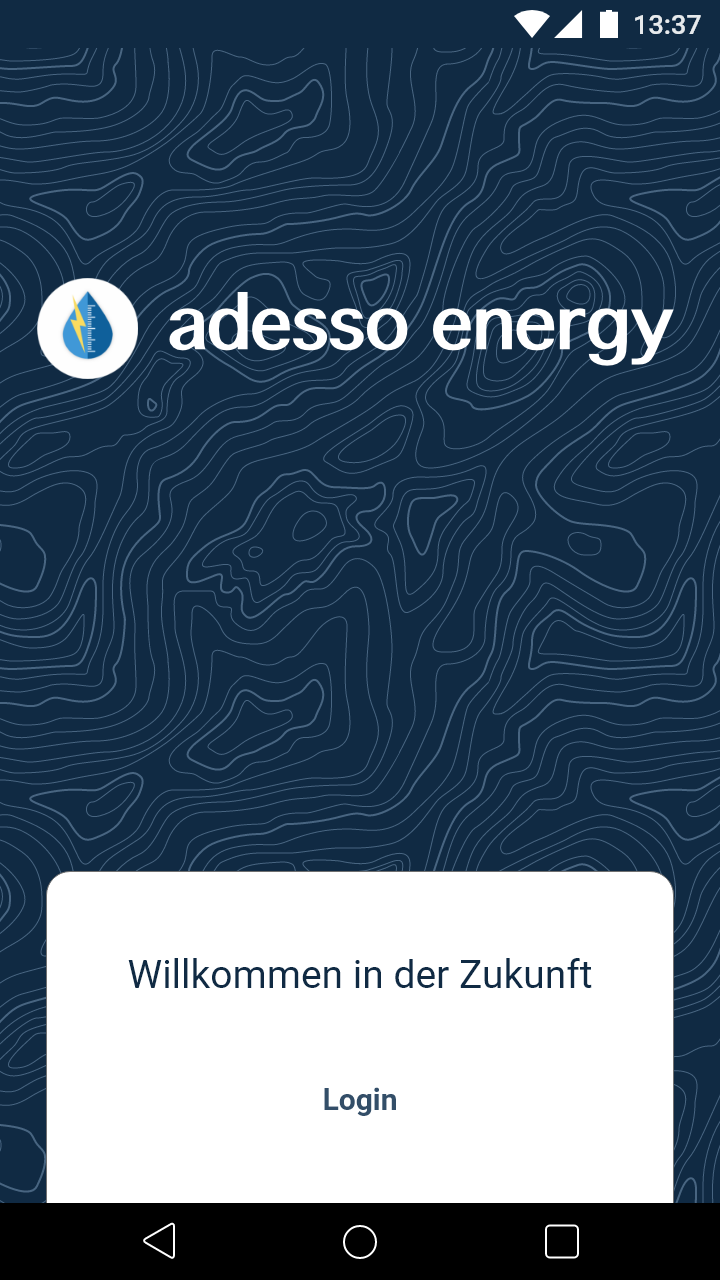
\includegraphics[scale = 0.155]{img/AndroidMockup/splash}  \caption {Startbildschirm} &  Dies ist der Bildschirm, den der Benutzer sieht, sobald er die App startet und noch nicht eingeloggt war.\\
	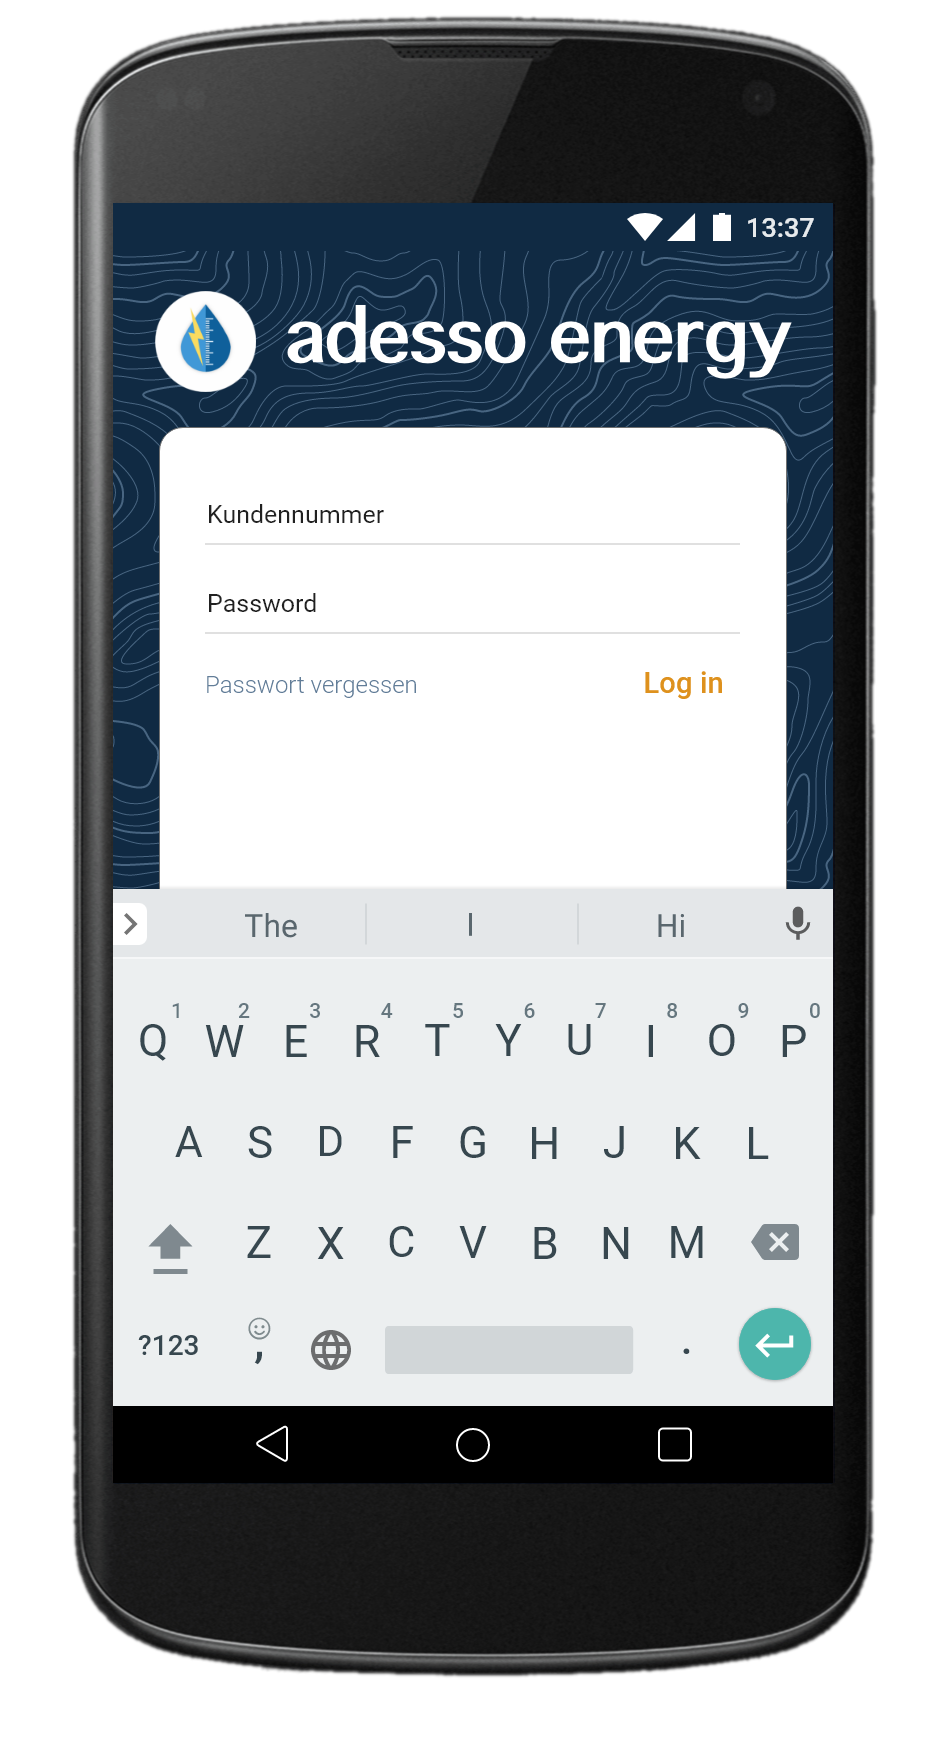
\includegraphics[scale = 0.155]{img/AndroidMockup/login} \caption {Anmeldebildschirm} &	Nachdem man auf dem Startbildschirm auf 'Log in' gedrückt hat, wird man auf den Anmeldebildschirm geleitet. Hier hat man die Möglichkeit, sich mit seiner Kundennummer und seinem Passwort einzuloggen. Außerdem hat man die Möglichkeit, mithilfe des 'Passwort vergessen'-Buttons, sein Passwort zurückzusetzen. \\ 
\end{tabularx}
\end{figure}


\begin{figure}[h]
\begin{tabularx}{\textwidth}{X  X}
	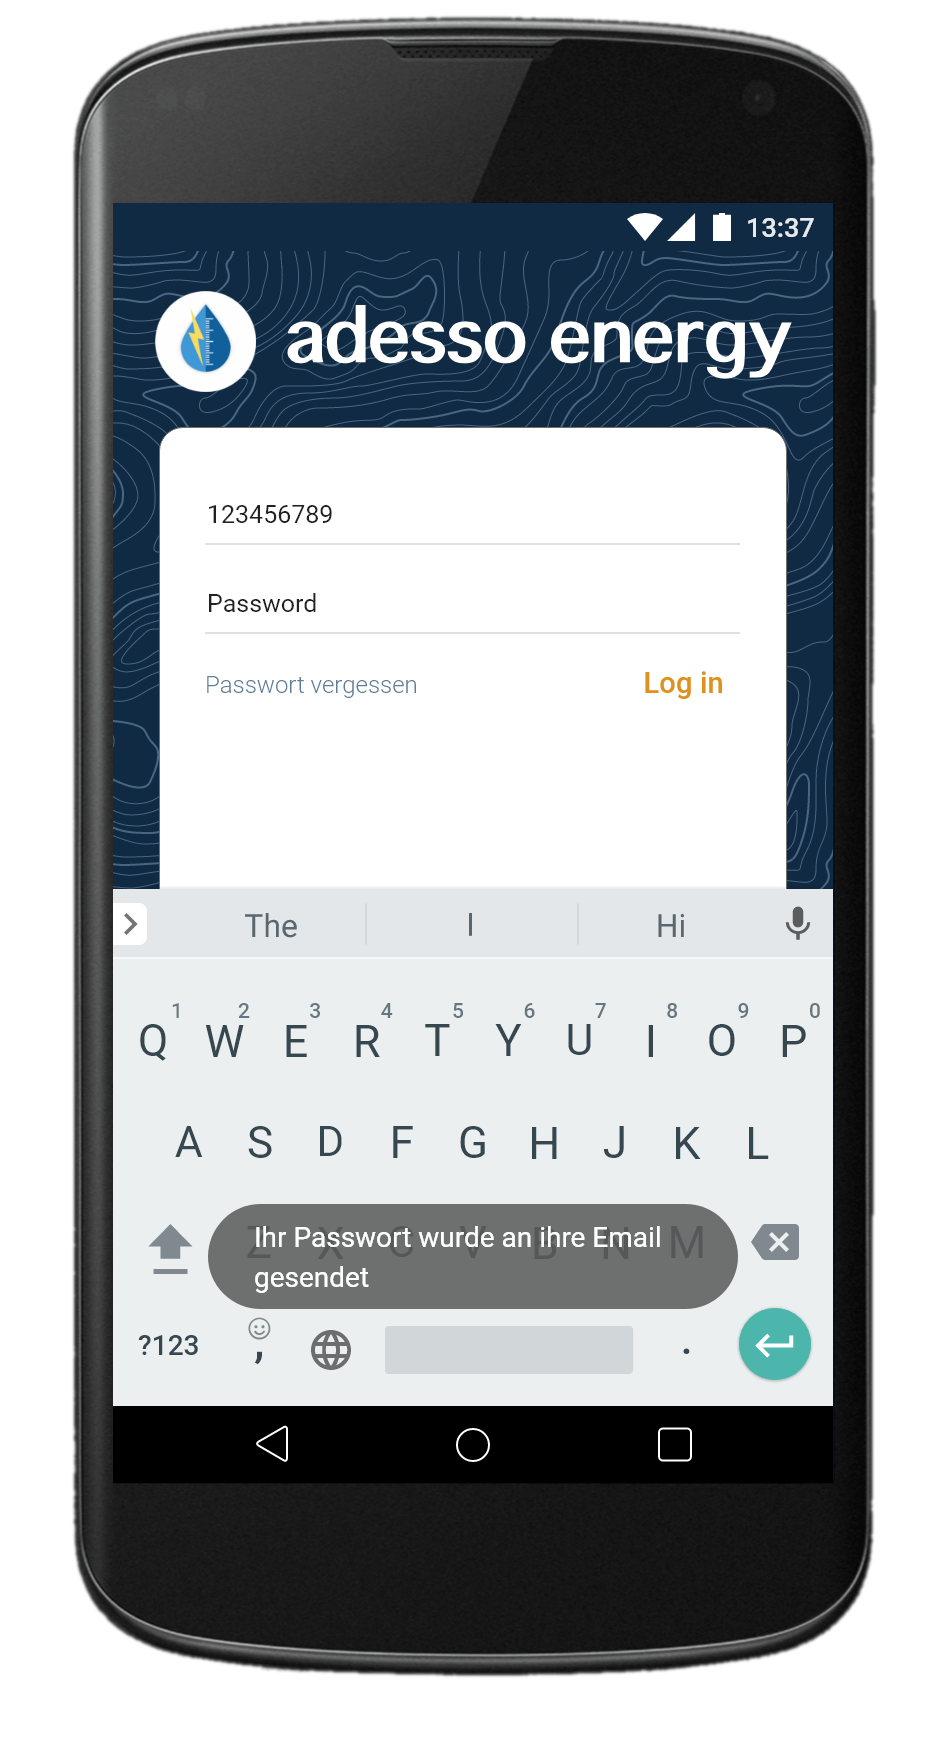
\includegraphics[scale = 0.155]{img/AndroidMockup/forgotPassword} \caption{Password vergessen} & Nachdem man auf 'Passwort vergessen' geklickt hat, erscheint eine Meldung, welche den Benutzer über das weitere Vorgehen informiert.\\
	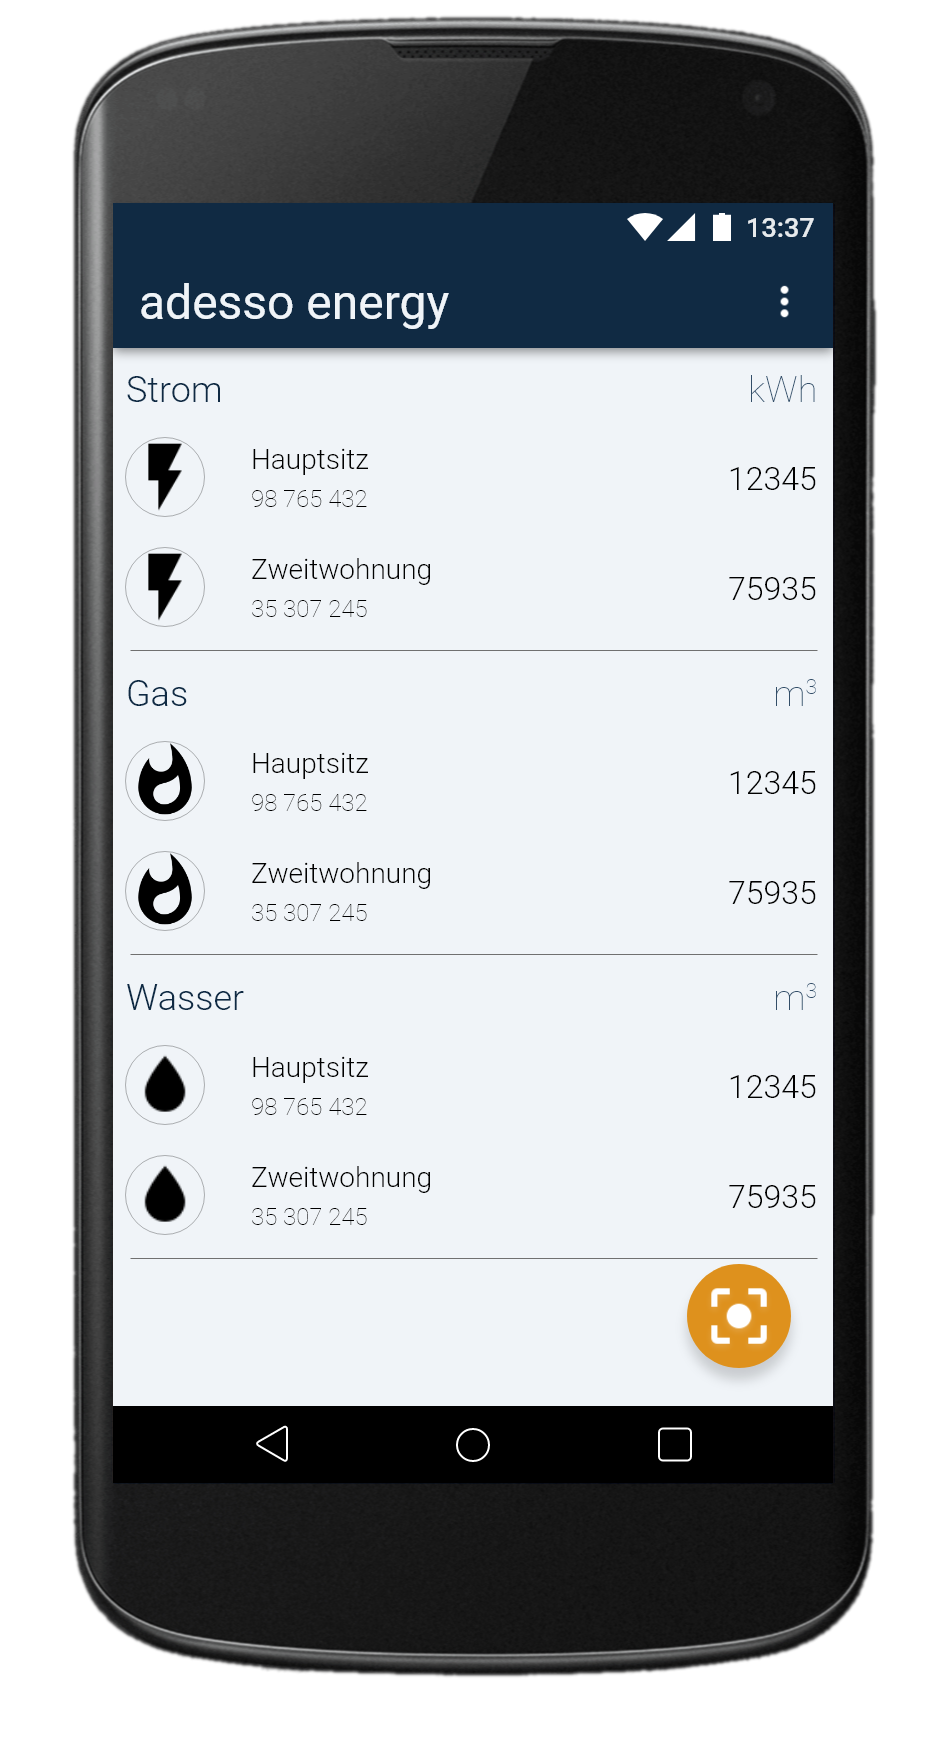
\includegraphics[scale = 0.155]{img/AndroidMockup/Main} \caption{Hauptbildschirm} & Nachdem man sich erfolgreich eingeloggt hat, landet man auf dem Hauptbildschirm. Hier sieht man eine Übersicht seiner Zähler mit deren Zählernummer und aktuellem Zählerstand. \\
\end{tabularx}
\end{figure}


\begin{figure}[h]
\begin{tabularx}{\textwidth}{X  X}
	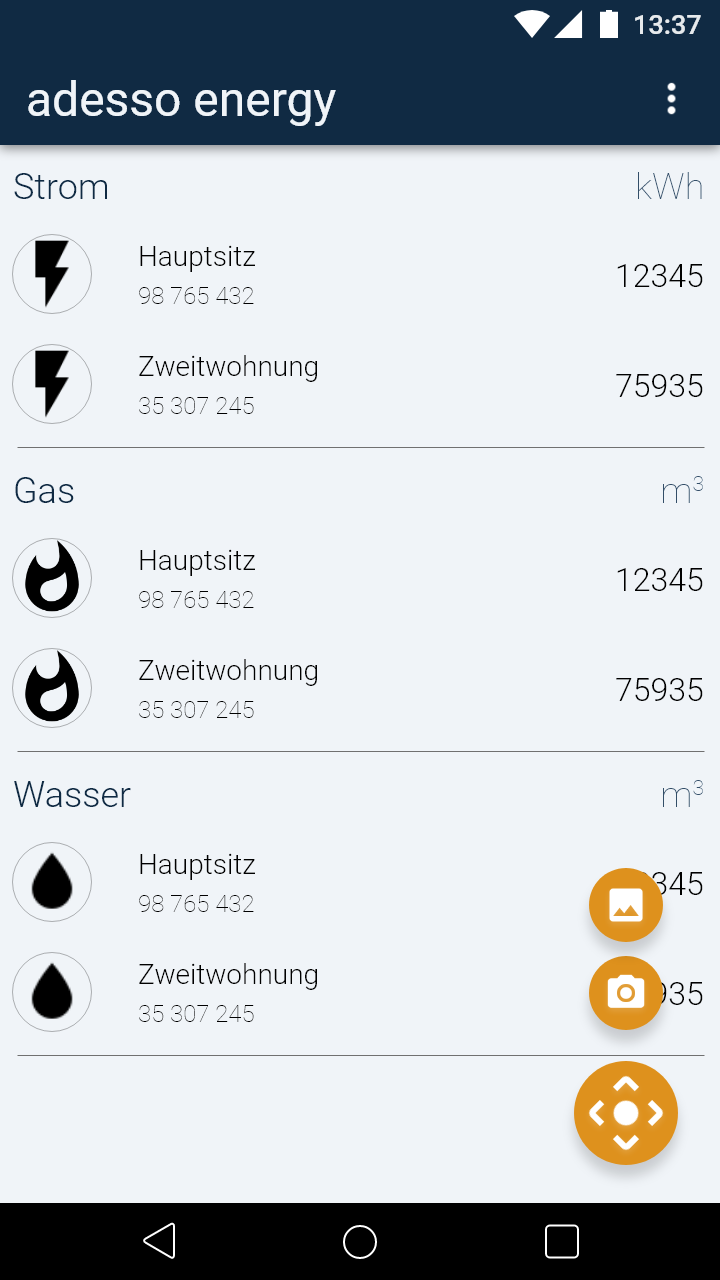
\includegraphics[scale = 0.155]{img/AndroidMockup/FABMenu} \caption{FAB-Menü}  & Klickt man auf den FAB, so erscheint ein Menü. Hier kann man sich entscheiden, ob man ein Bild aufnehmen möchte (Kamera-Symbol) oder eines aus der Galerie hochladen möchte (Galerie-Symbol). \\
	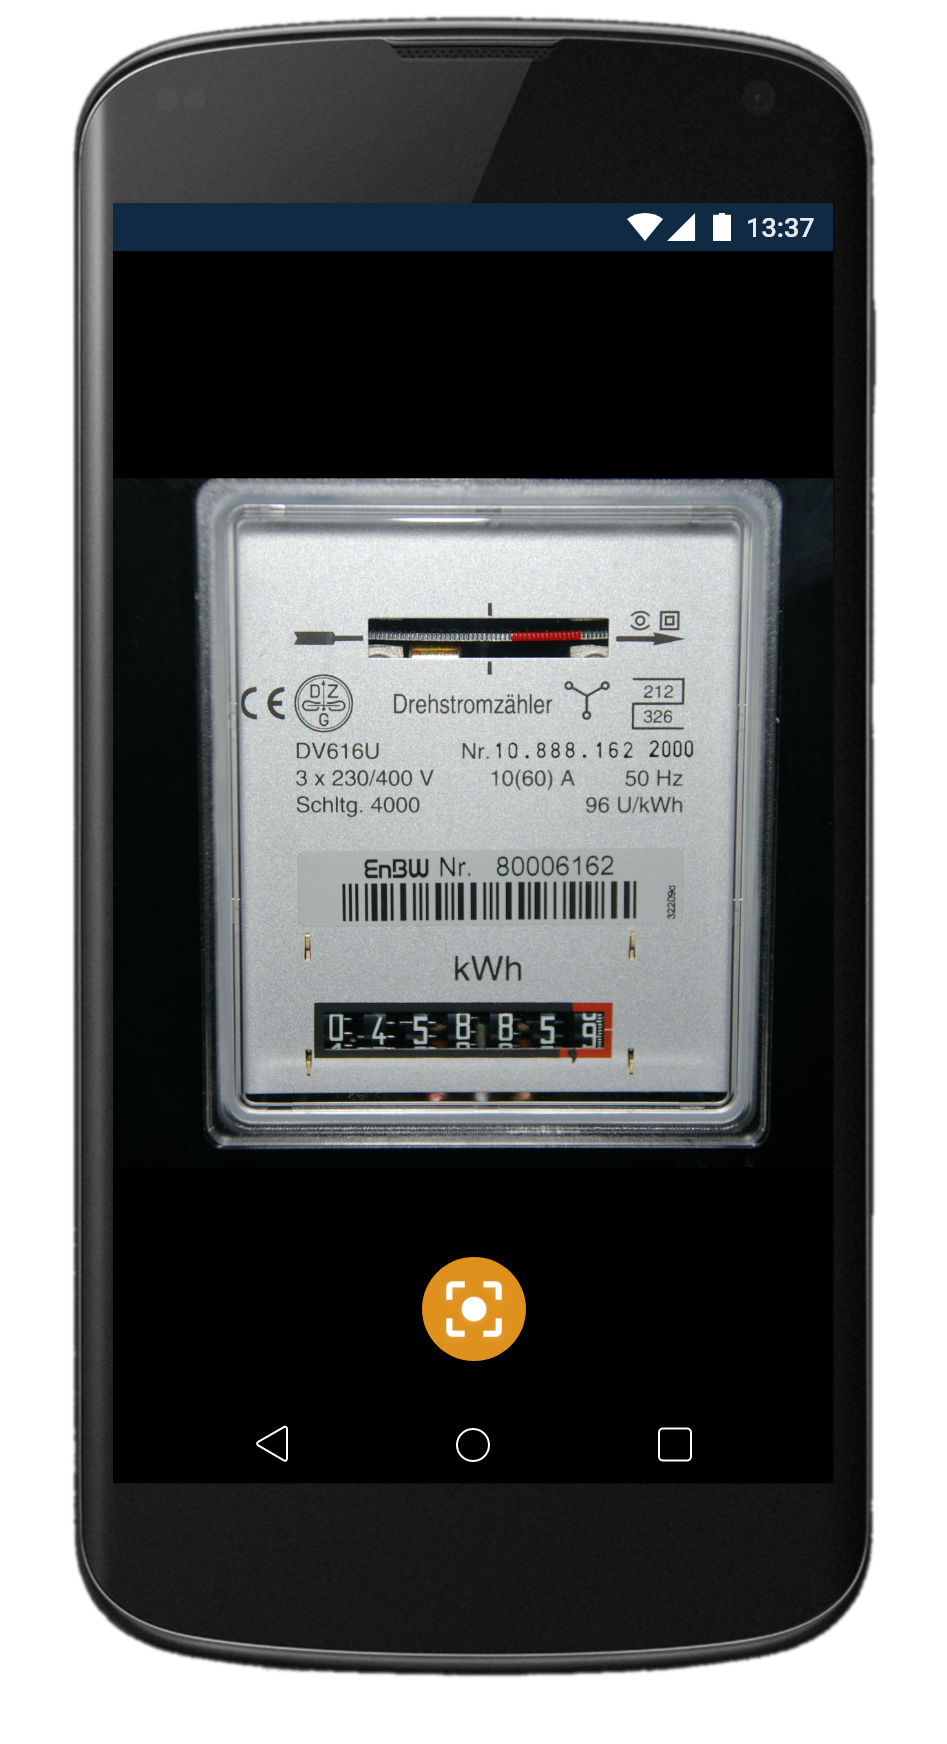
\includegraphics[scale = 0.155]{img/AndroidMockup/SystemCamera} \caption{Kamera-View}  & Nachdem man im Dropdown Menü das Kamera-Symbol gedrückt hat, öffnet sich die Kamera-App des Gerätes. \\ 
\end{tabularx}
\end{figure}

\begin{figure}[h]
\begin{tabularx}{\textwidth}{X  X}
	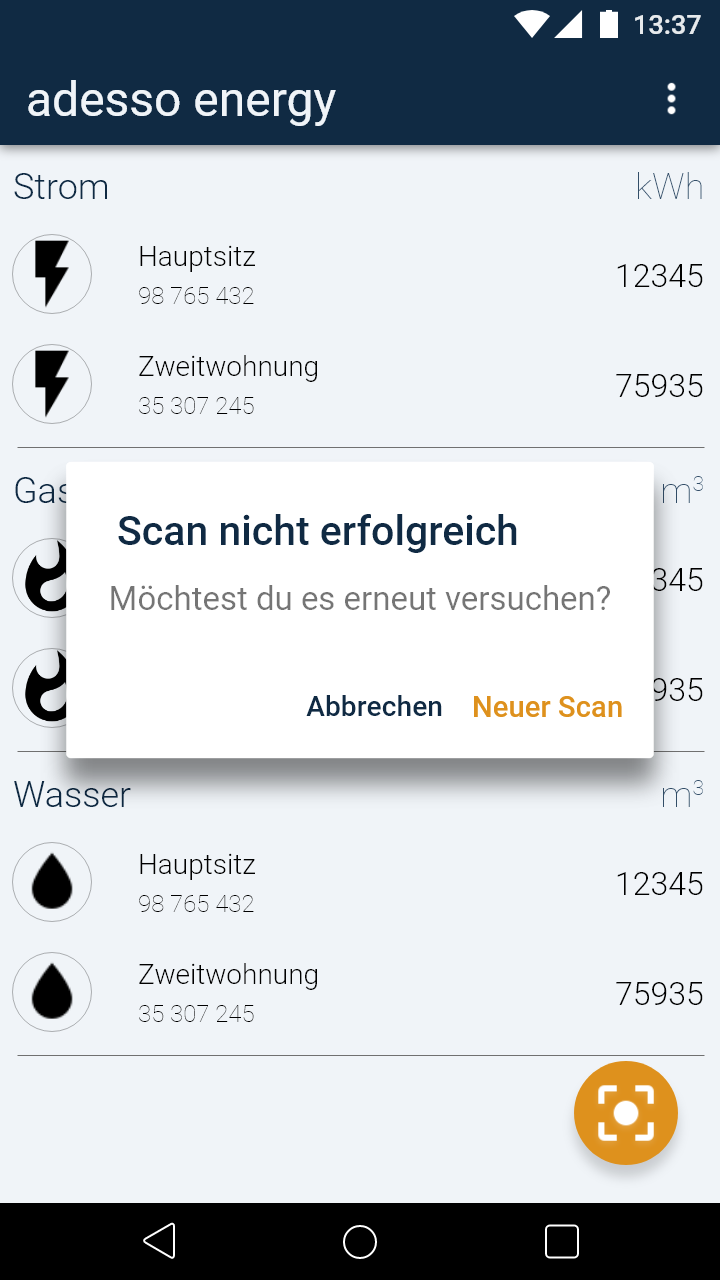
\includegraphics[scale = 0.155]{img/AndroidMockup/imageFailed} \caption{Scan fehlgeschlagen} & Wurde auf dem Bild kein Zähler erkannt, so erscheint eine entsprechende Meldung. Hier hat man die Möglichkeit, erneut ein Foto zu machen oder den Vorgang abzubrechen. \\
	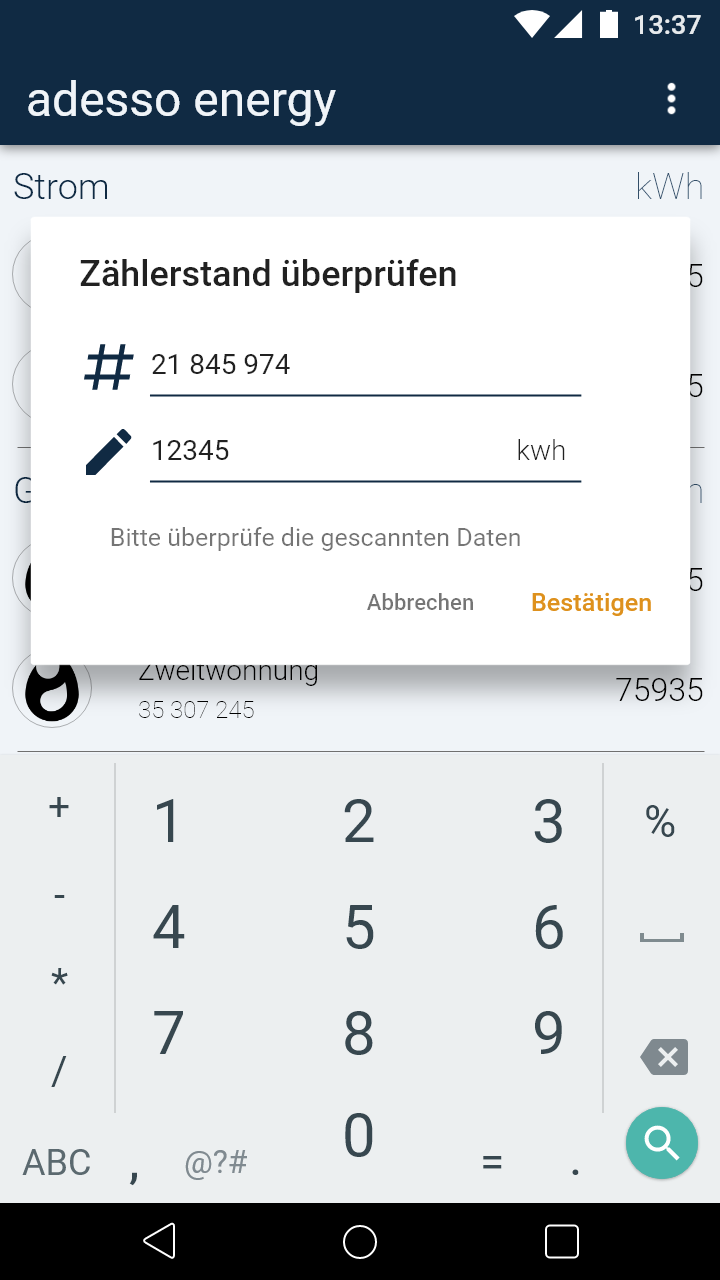
\includegraphics[scale = 0.155]{img/AndroidMockup/check} \caption{Werte überprüfen} & Wurde ein Foto erfolgreich verarbeitet, so folgt eine Überprüfung der Werte, welche von Azure erkannt wurden. Vor dem endgültigen Speichern der Werte müssen diese vom Benutzer bestätigt werden. \\ 
\end{tabularx}
\end{figure}

\begin{figure}[h]
\begin{tabularx}{\textwidth}{X  X}
	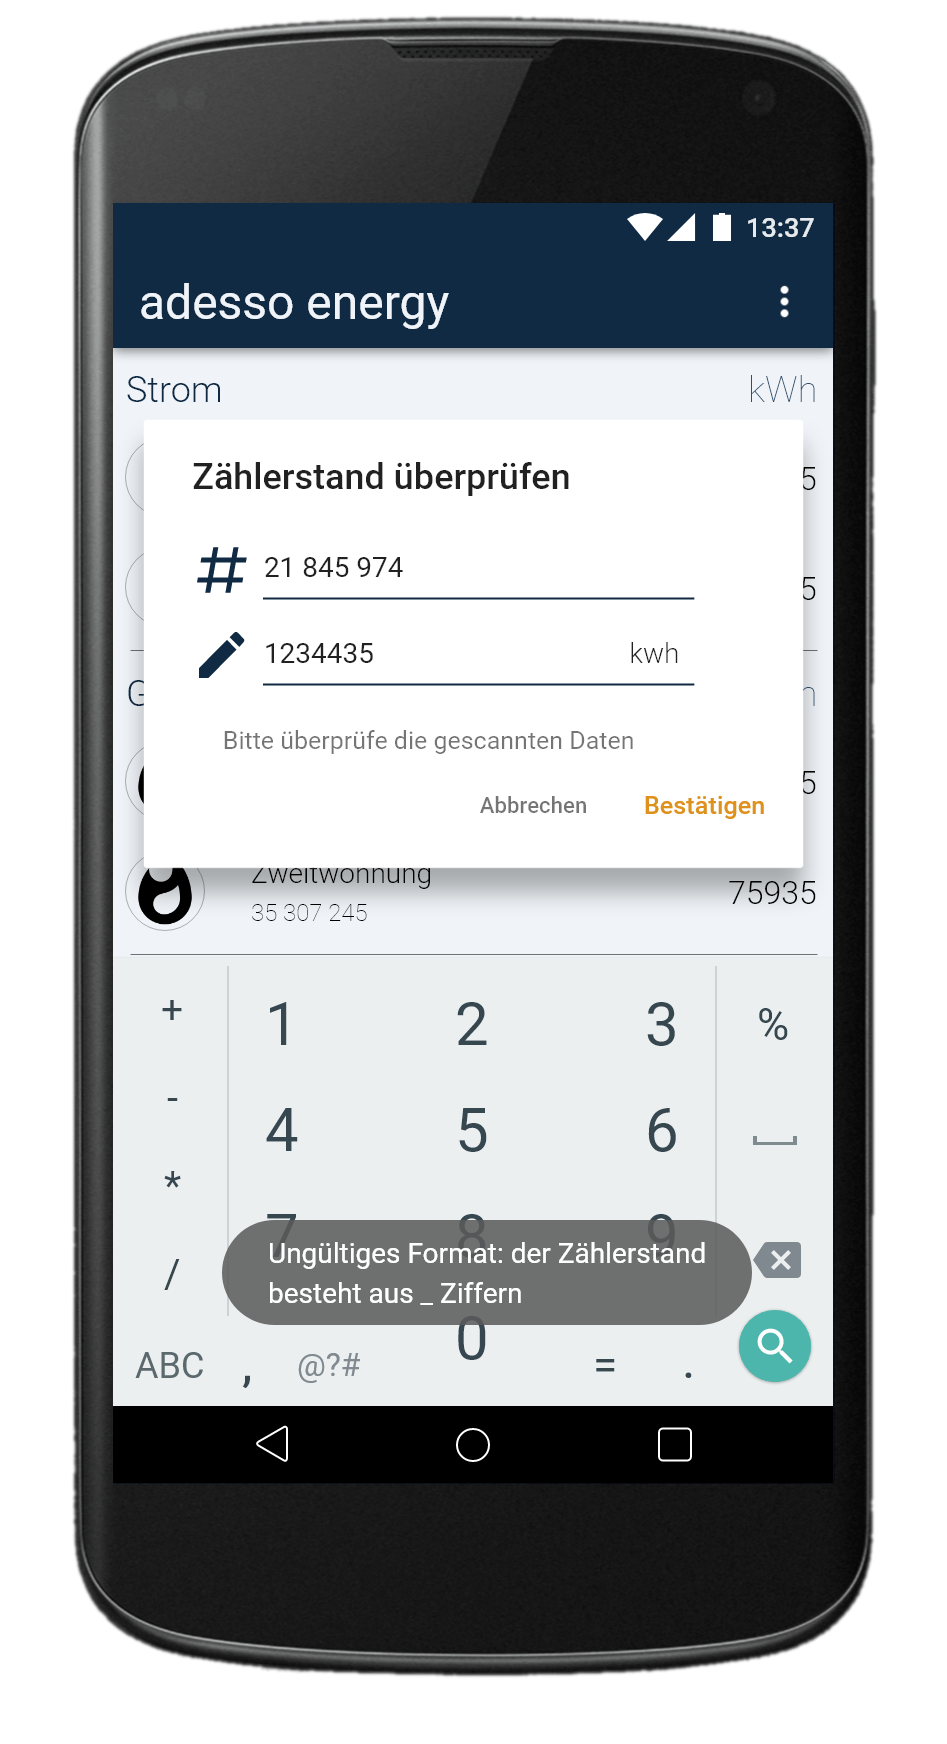
\includegraphics[scale = 0.155]{img/AndroidMockup/illegalFormatException} \caption{Falsches Zahlenformat} & Gibt man Werte in einem falschem Format ein, so erhält man eine entsprechende Meldung. \\
	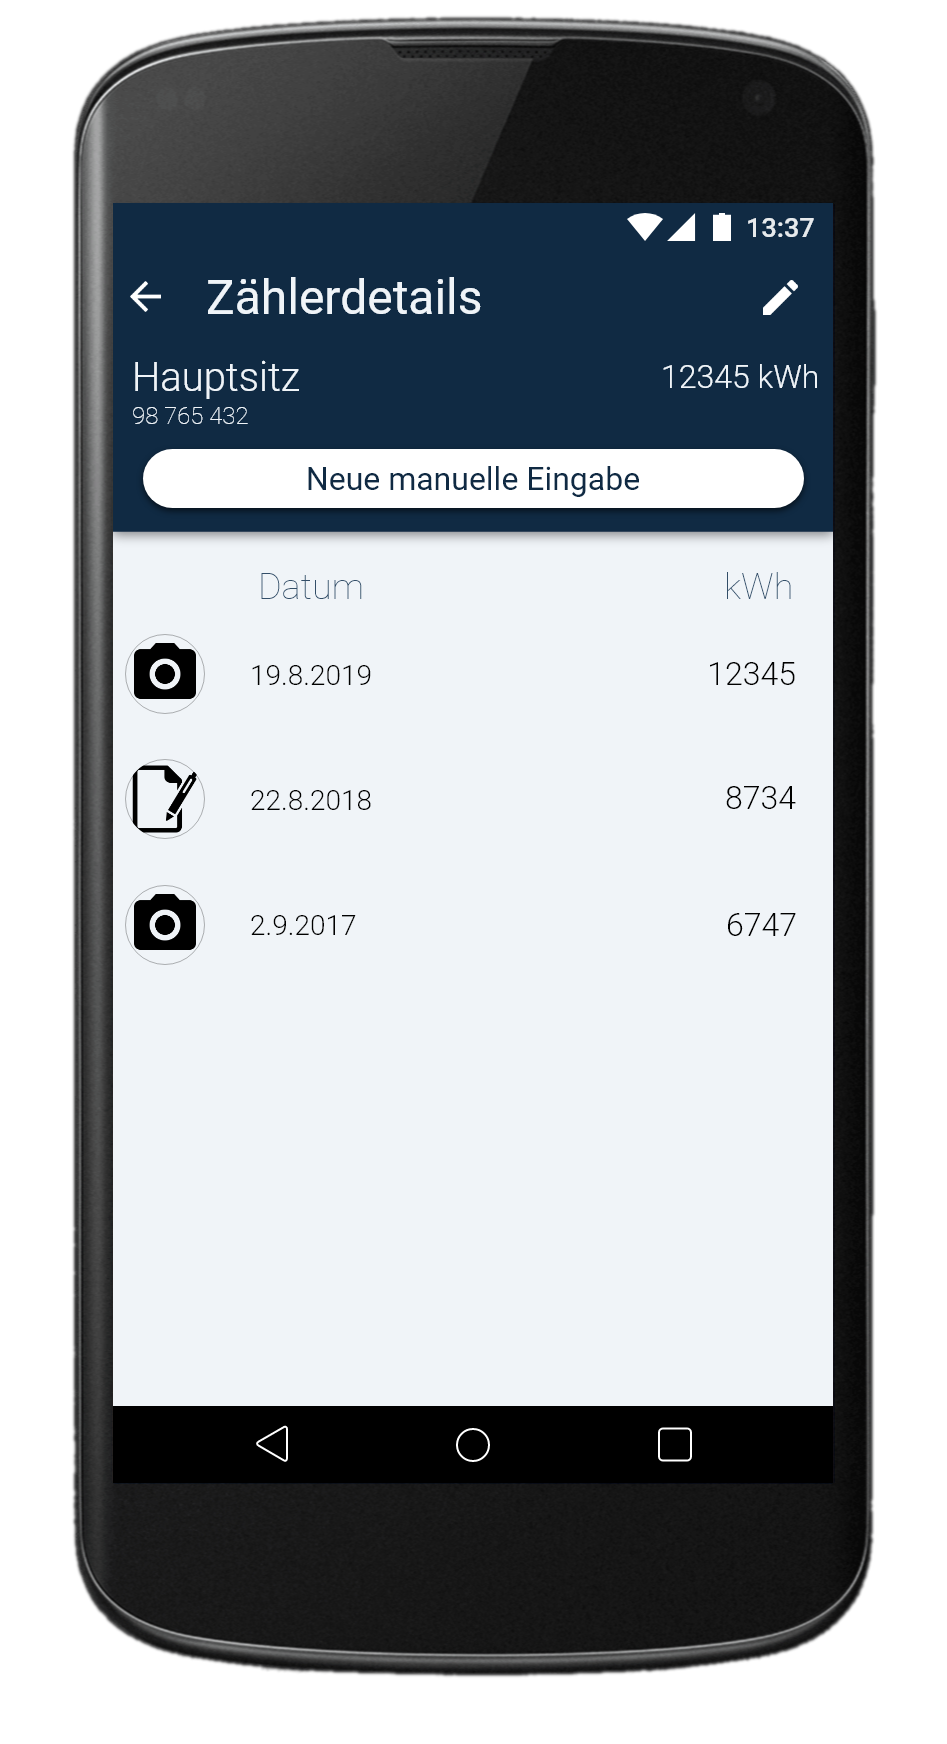
\includegraphics[scale = 0.155]{img/AndroidMockup/history} \caption{Zählerstand-Details} & Klickt man auf einen der Zähler, so sieht man die gesamte History der eingetragenen Zählerstände. Außerdem sieht man, wann der Zählerstand hochgeladen worden ist und ob dies durch eine manuelle Eingabe oder per Foto geschah. \\
\end{tabularx}
\end{figure}

\begin{figure}[h]
\begin{tabularx}{\textwidth}{X  X}
	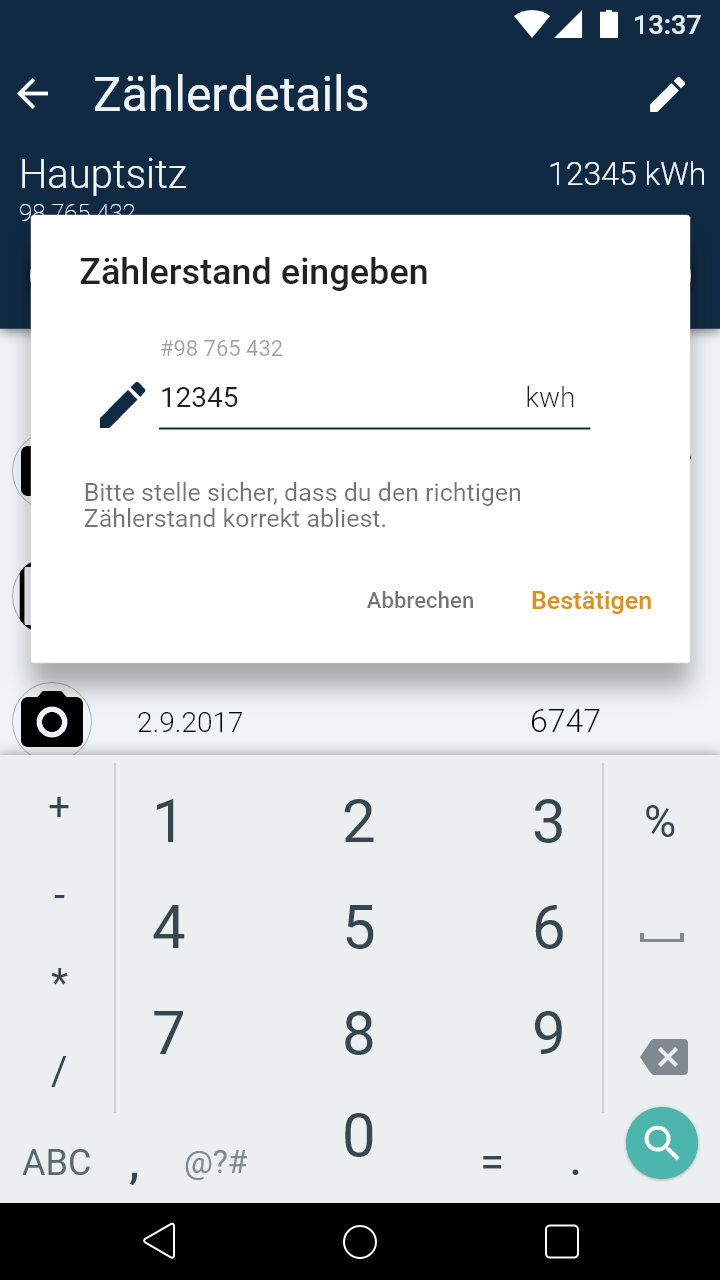
\includegraphics[scale = 0.155]{img/AndroidMockup/manuelEntry} \caption{Manueller Eintrag}&  Sobald der Zähler ausgewählt ist, hat man die Möglichkeit, manuell einen Zählerstand einzutragen. \\
	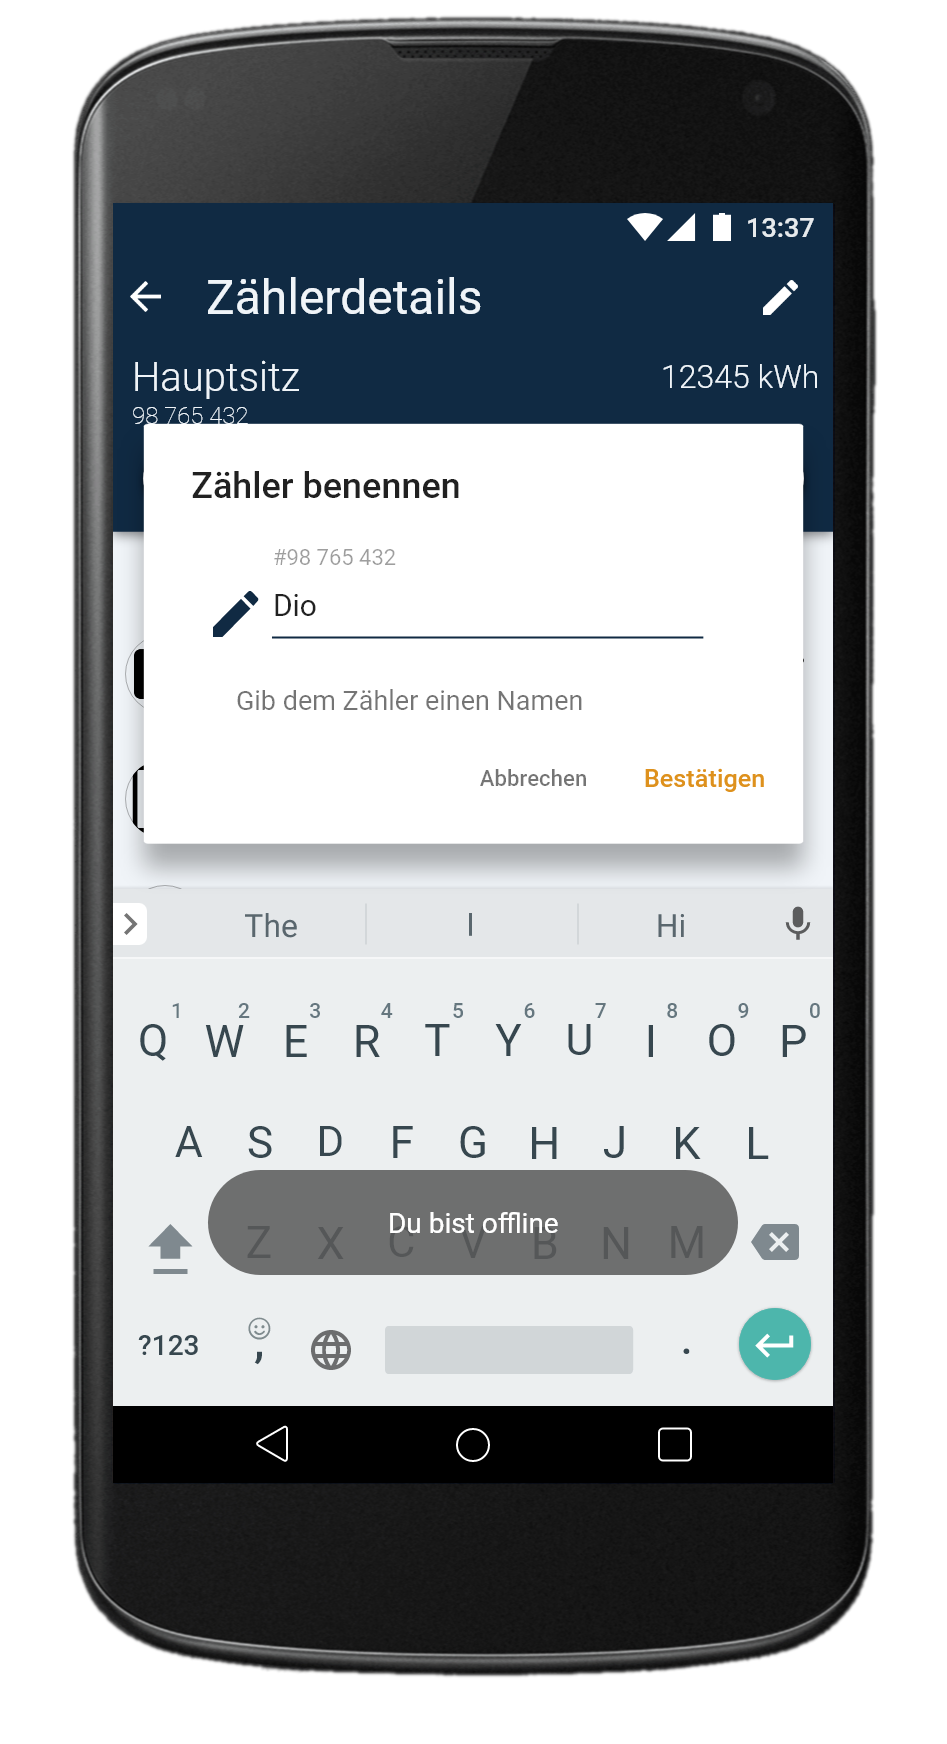
\includegraphics[scale = 0.155]{img/AndroidMockup/renameException} \caption{Offline-Meldung} & Verliert man während eines Vorganges seine Internetverbindung, so erscheint eine entsprechende Meldung und der Vorgang wird nicht durchgeführt.  \\ 
\end{tabularx}
\end{figure}

\begin{figure}[h]
\begin{tabularx}{\textwidth}{X  X}
	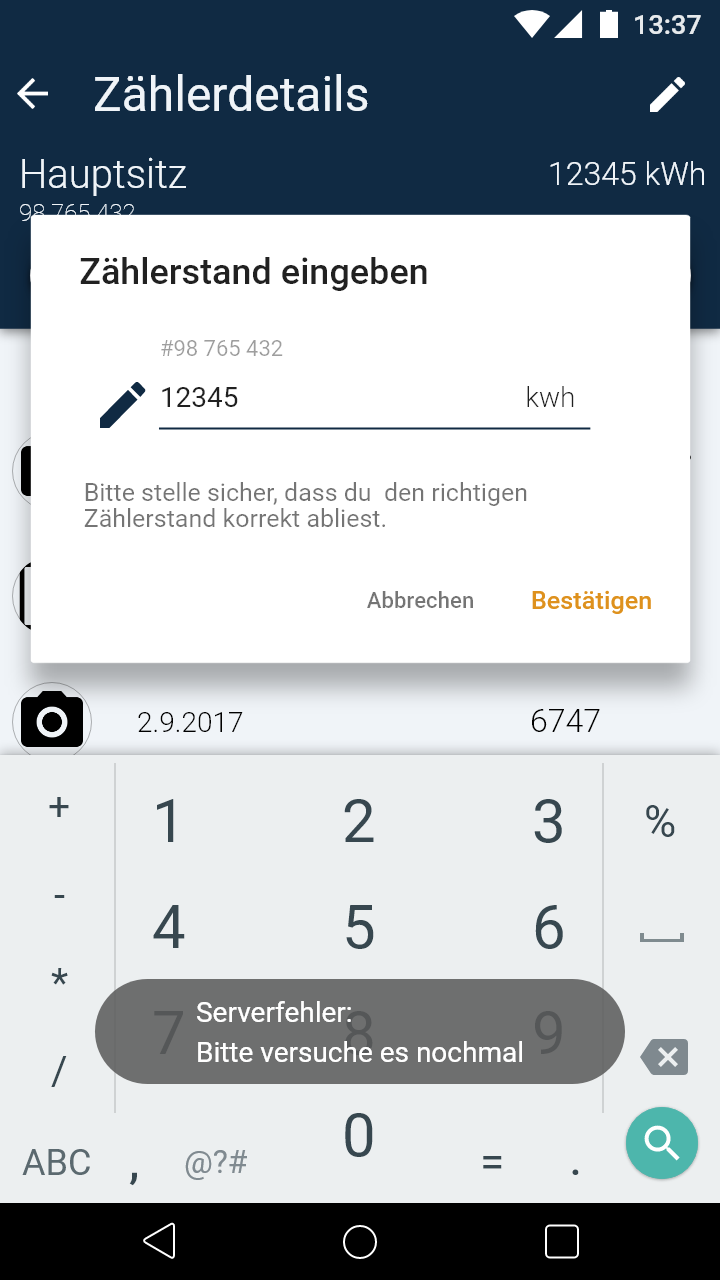
\includegraphics[scale = 0.155]{img/AndroidMockup/serverException} \caption{Serverfehler} & Falls während der Ausführung eines Vorganges ein Serverproblem geschieht, so erscheint eine entsprechende Meldung und der Vorgang wird nicht durchgeführt.\\
	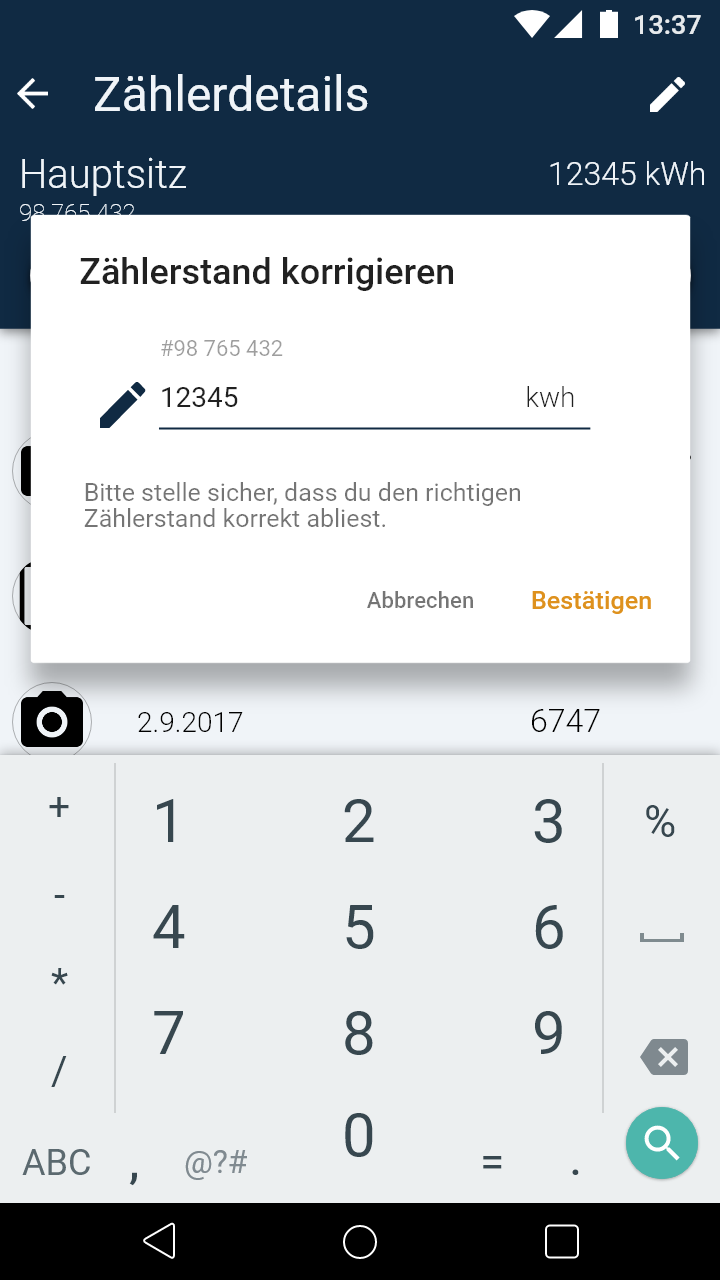
\includegraphics[scale = 0.155]{img/AndroidMockup/correct} \caption{Zählerstand korrigieren} & Wurde ein falscher Zählerstand eingetragen, so hat man nachträglich die Möglichkeit, ihn zu korrigieren.\\ 
\end{tabularx}
\end{figure}

\begin{figure}[h]
\begin{tabularx}{\textwidth}{X  X}
	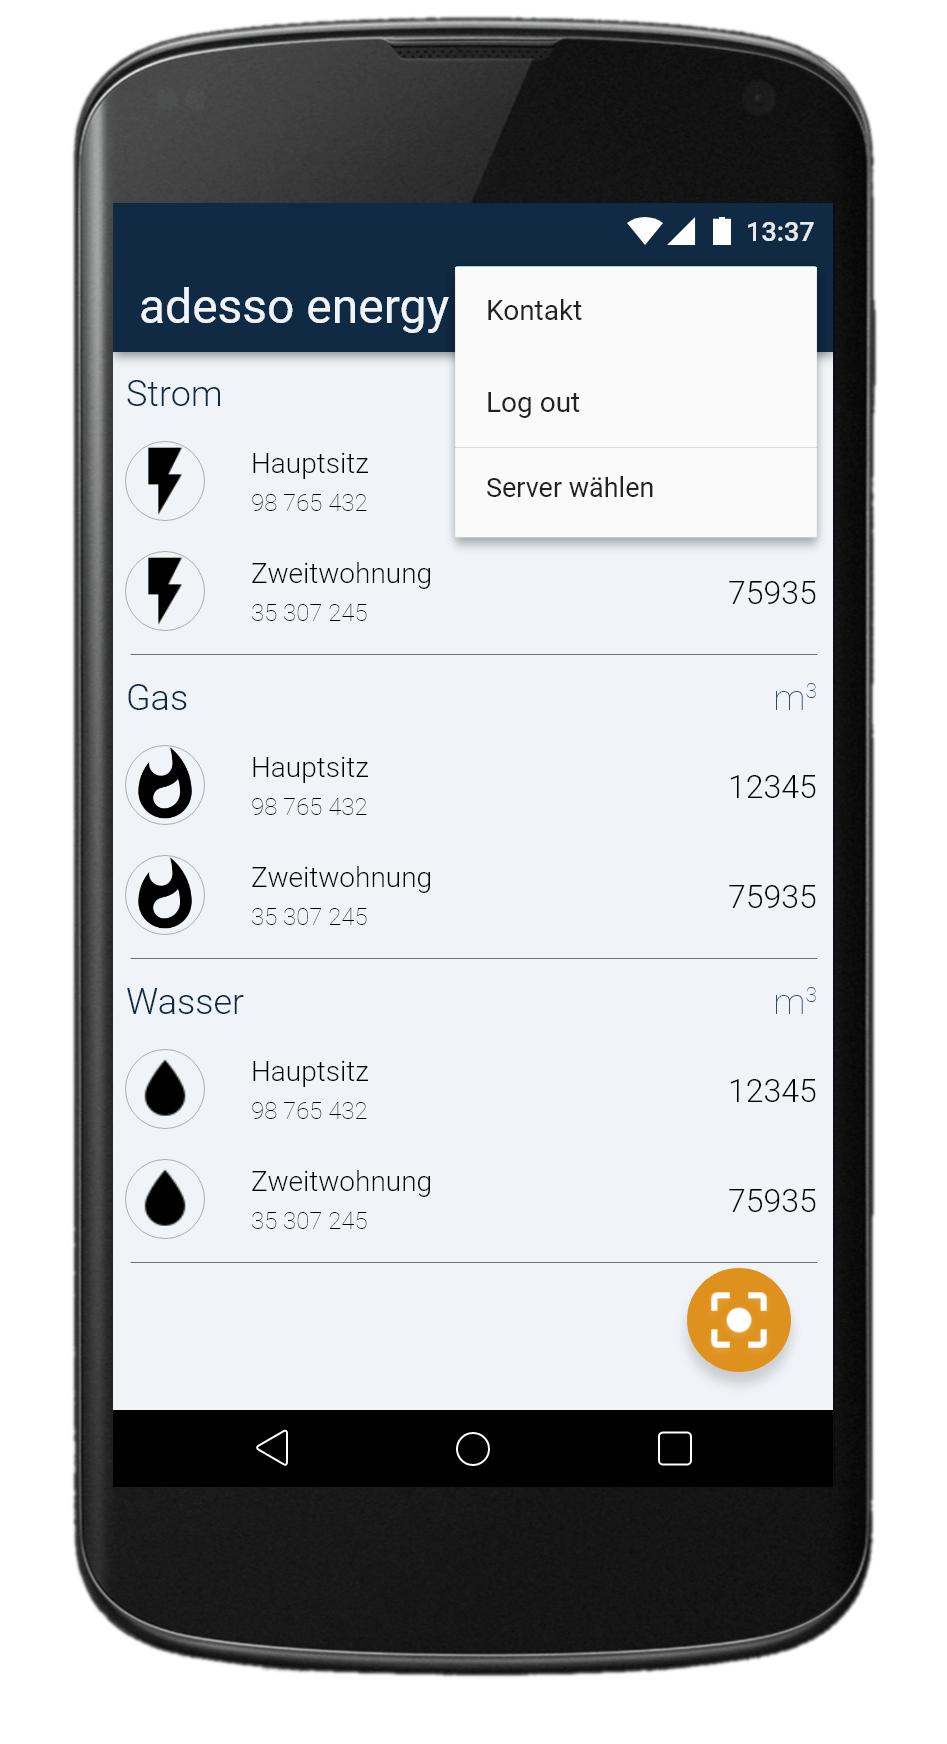
\includegraphics[scale = 0.155]{img/AndroidMockup/dropdown} \caption{Dropdown-Menü} & Man hat auf dem Startbildschirm außerdem die Möglichkeit, oben rechts ein Dropdown-Menü zu öffnen. Hier hat man die Möglichkeit, die Adresse des Servers auszuwählen, sich abzumelden, sowie Kontakt zum Support aufzunehmen. \\
	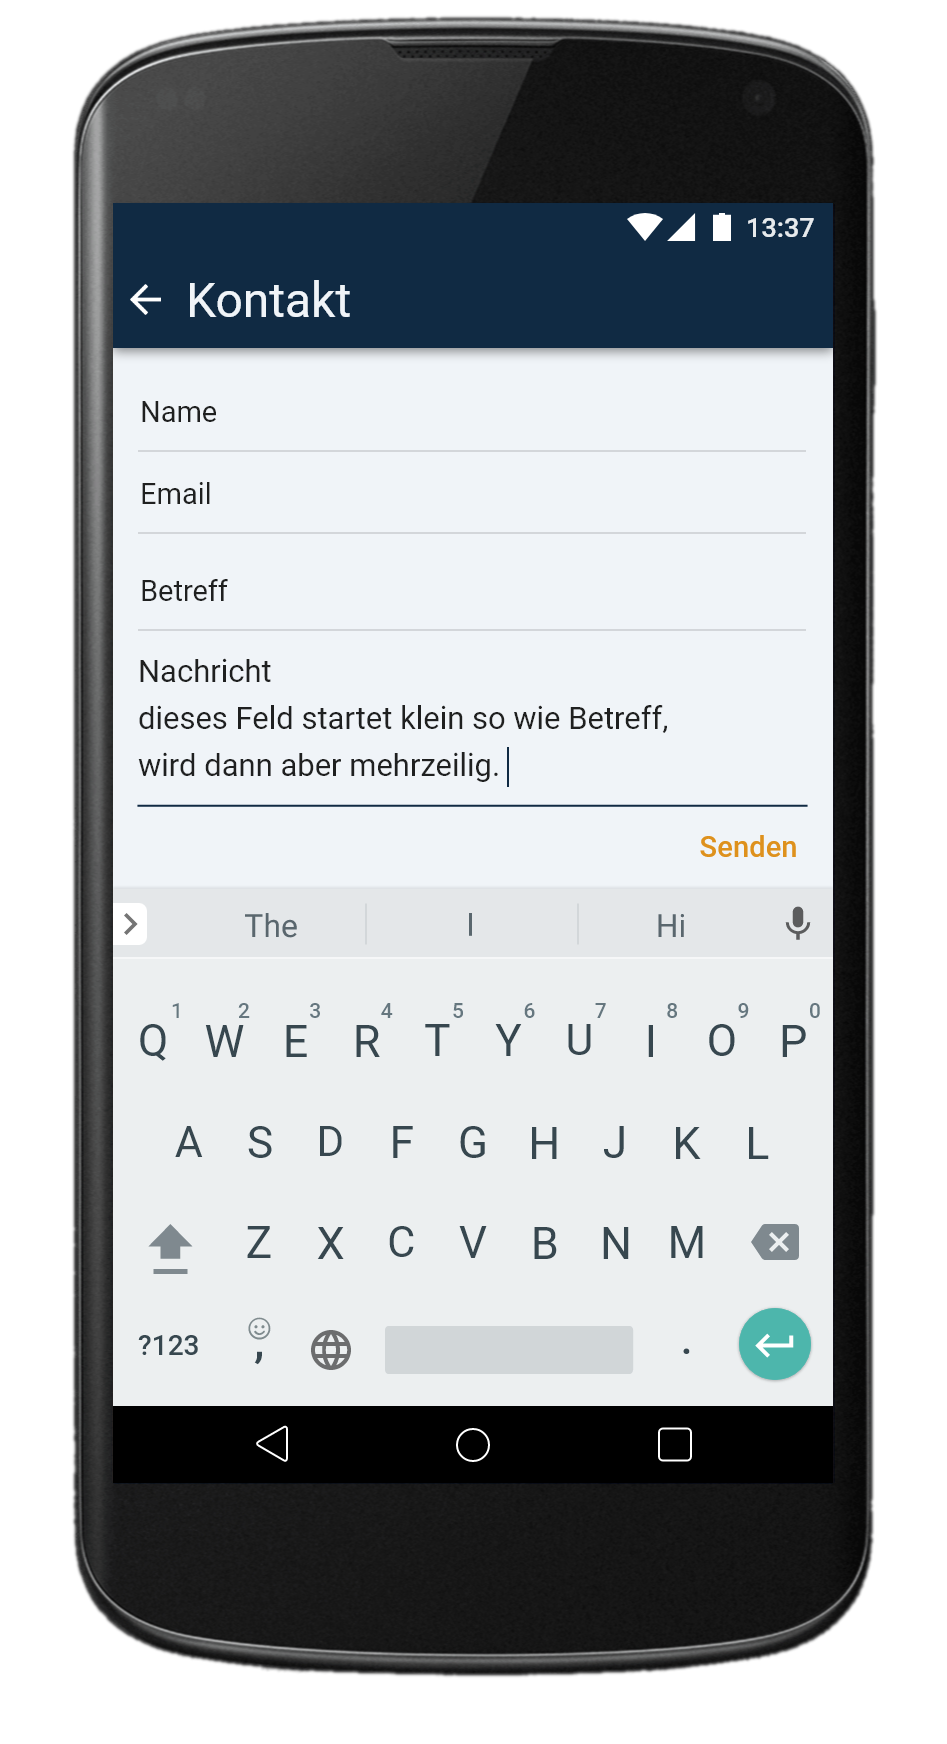
\includegraphics[scale = 0.155]{img/AndroidMockup/contact} \caption{Kontaktformular} & Sobald man sich entschieden hat, Kontakt mit dem Support aufzunehmen, erscheint ein Kontaktformular. Hier soll der Benutzer seinen Namen, seine e-Mail-Adresse, den Betreff und eine Nachricht angeben. \\ 
\end{tabularx}
\end{figure} 

\begin{figure}[h]
\begin{tabularx}{\textwidth}{X  X}
	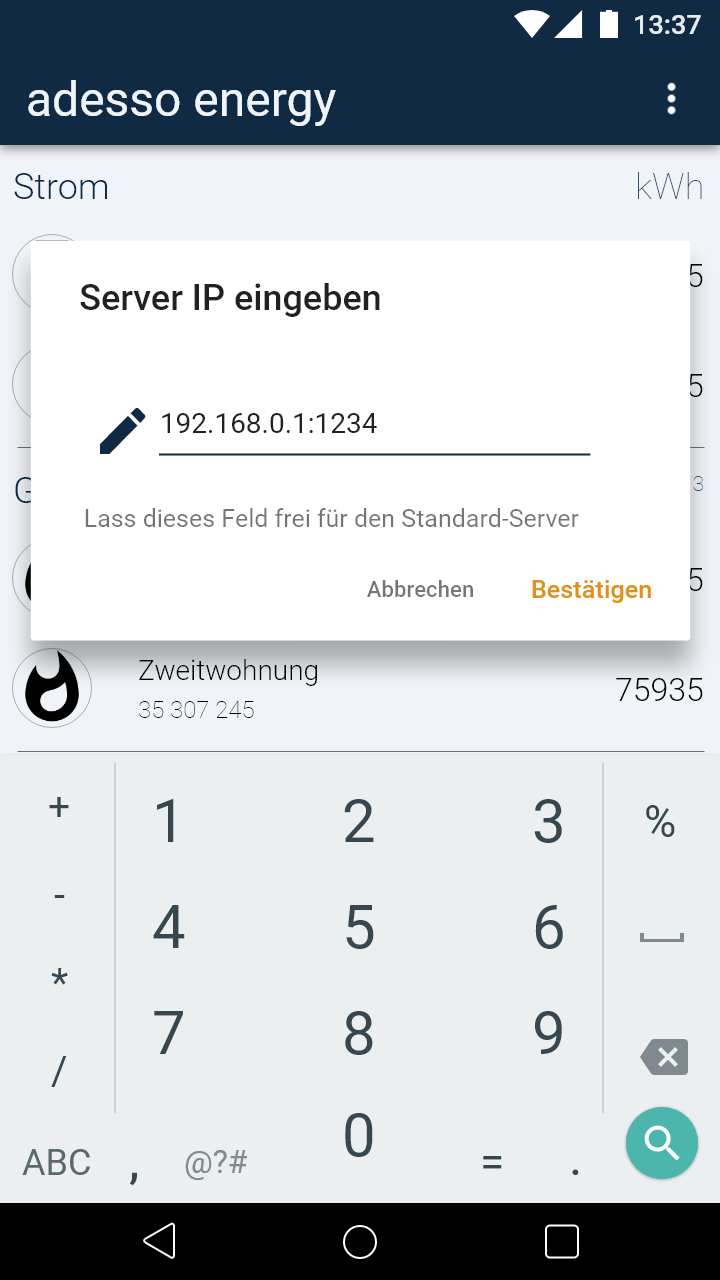
\includegraphics[scale = 0.155]{img/AndroidMockup/serverLocation} \caption{Server wählen} & Möchte man die Adresse des Servers ändern, so klickt man auf 'Server wählen'. Hier hat man die Möglichkeit, einen Servers mithilfe seiner IP-Adresse zu bestimmen und auf diesen zu wechseln. \\
	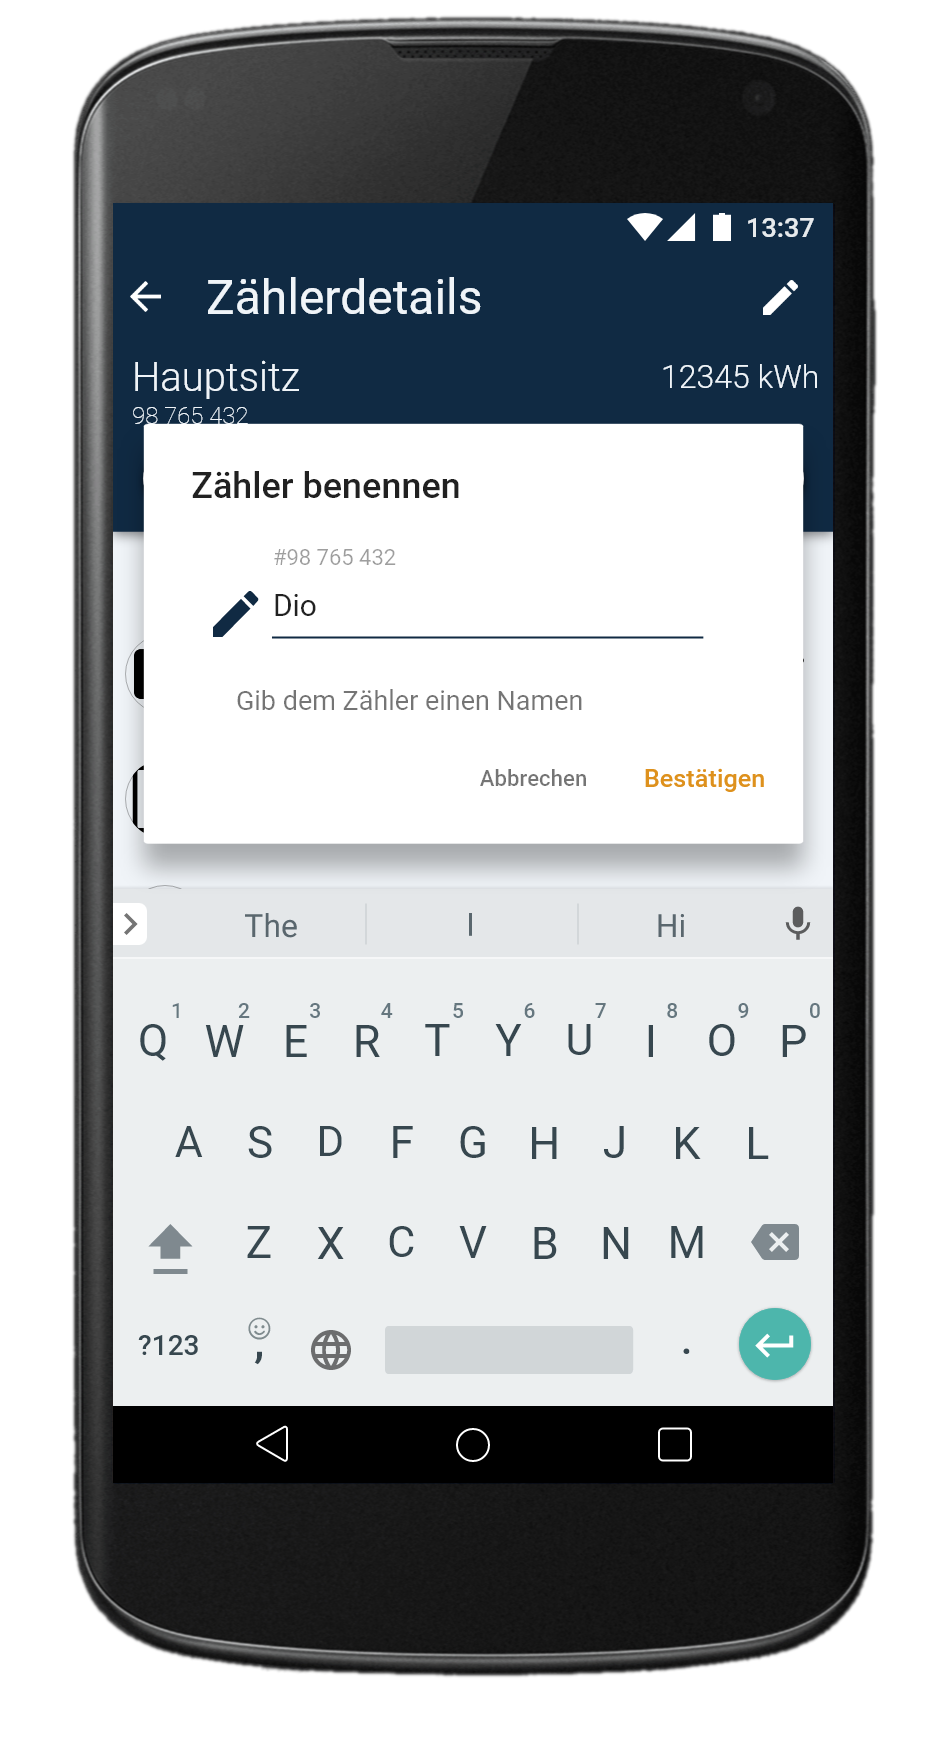
\includegraphics[scale = 0.155]{img/AndroidMockup/rename} \caption{Zähler umbenennen} & Wenn der Benutzer einen Zähler aus dem Hauptbildschirm ausgewählt hat, hat er die Möglichkeit, diesem zur einfacheren Identifikation einen Namen zuzuweisen. \\
\end{tabularx}
\end{figure}

% Section Web

\newpage

\begin{figure}[h] 
	\newpage
	\section{Web Mockup}

	In diesem Abschnitt werden die Mockups der Webseite vorgestellt, welche in interaktiver Form auch hier zu finden sind:
	\url{https://www.figma.com/file/Eyt5hgvjWapVjybG8g21tF/Website?node-id=0%3A1} .

	\centering
    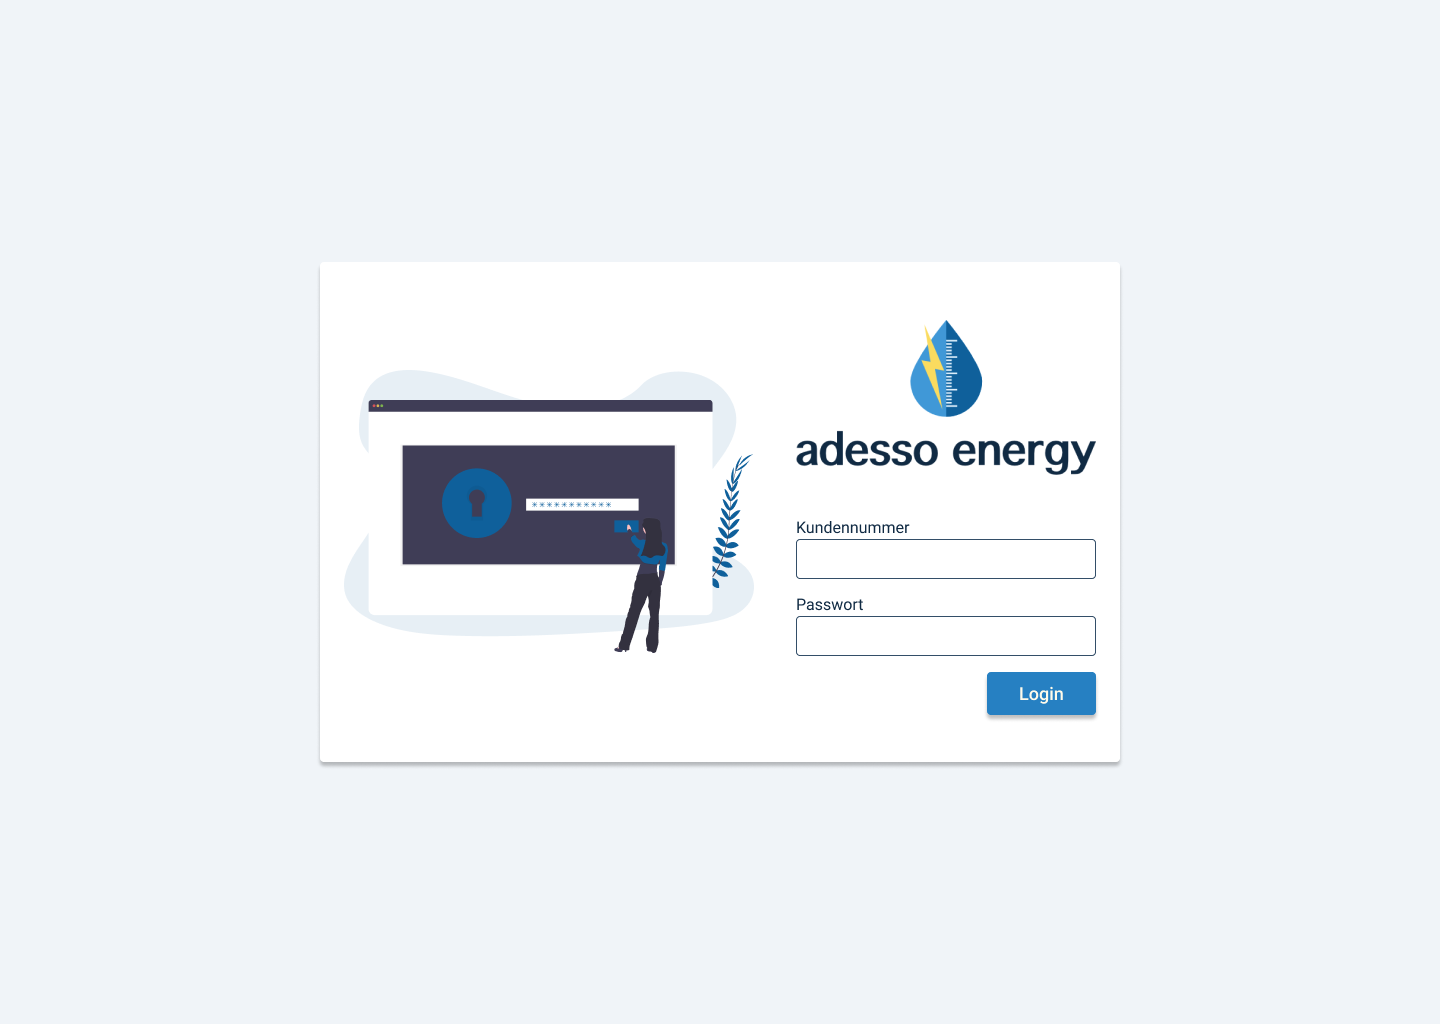
\includegraphics[scale=0.3]{img/WebsiteMockup/Login-User}
	\caption{Login Bildschirm} \hfill \break
	Hier sieht man den Login Screen in dem sich User und Admins mithilfe von Kundennummer und Passwort anmelden kann.
\end{figure}
 
\newpage

\begin{figure}[h]
	\centering
    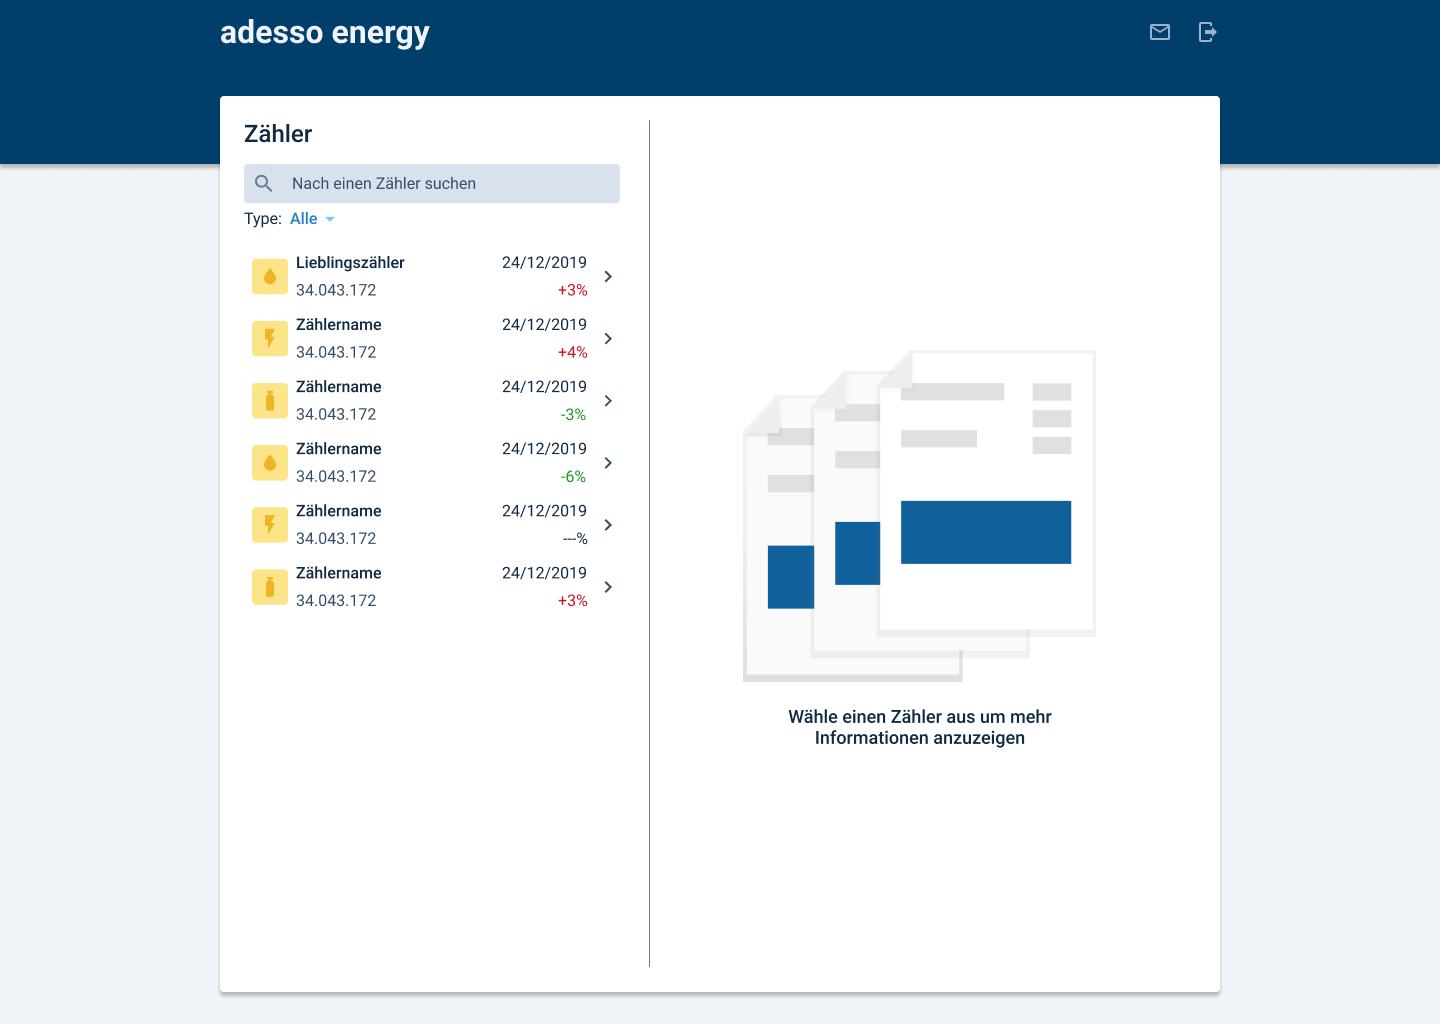
\includegraphics[scale=0.3]{img/WebsiteMockup/Dashboard-User-NonSelected}
	\caption{Dashboard User} \hfill \break
	Nachdem man sich erfolgreich eingeloggt wird man auf den Startbildschirm weitergeleitet. Hier kann der Benutzer seine Zähler einsehen.
\end{figure}

\newpage

\begin{figure}[h]
	\centering
    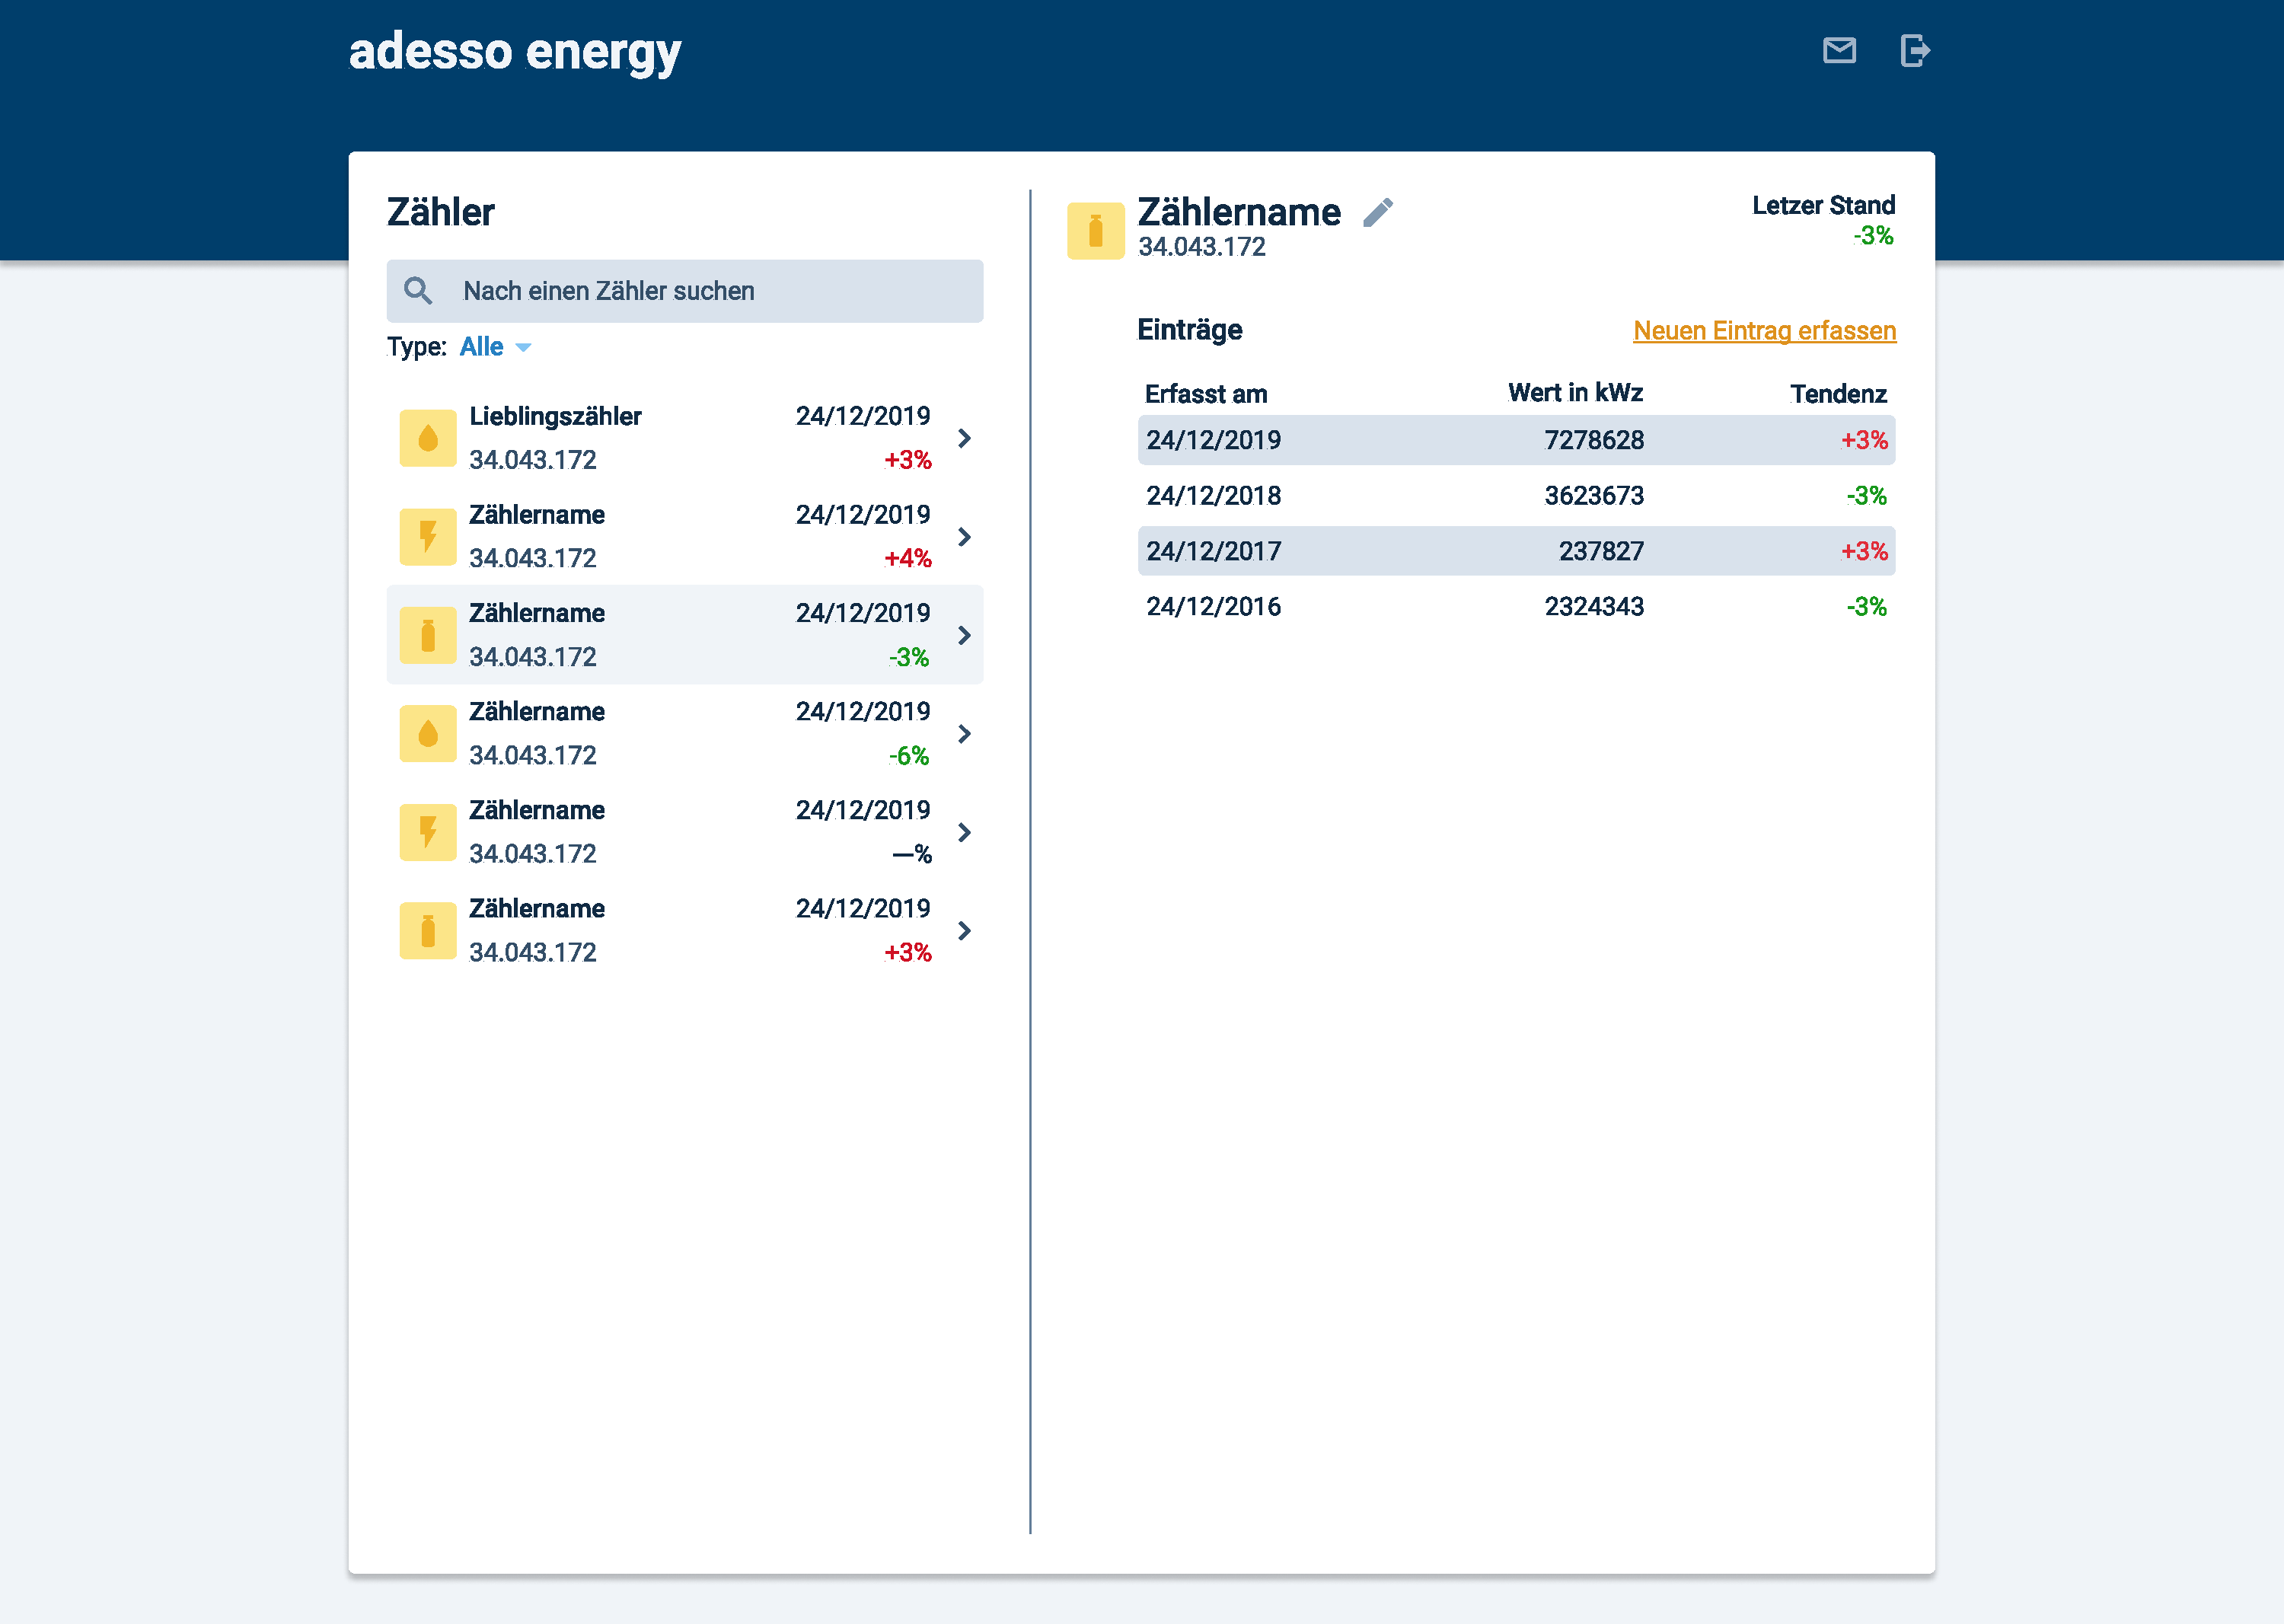
\includegraphics[scale=0.3]{img/WebsiteMockup/Dashboard-User-Selected}
	\caption{Dashboard User mit ausgewähltem Zähler} \hfill \break
	Nachdem man einen Zähler ausgewählt hat, sieht man seine History mit Datum und Zählerstand.
\end{figure}

\newpage

\begin{figure}[h]
	\centering
    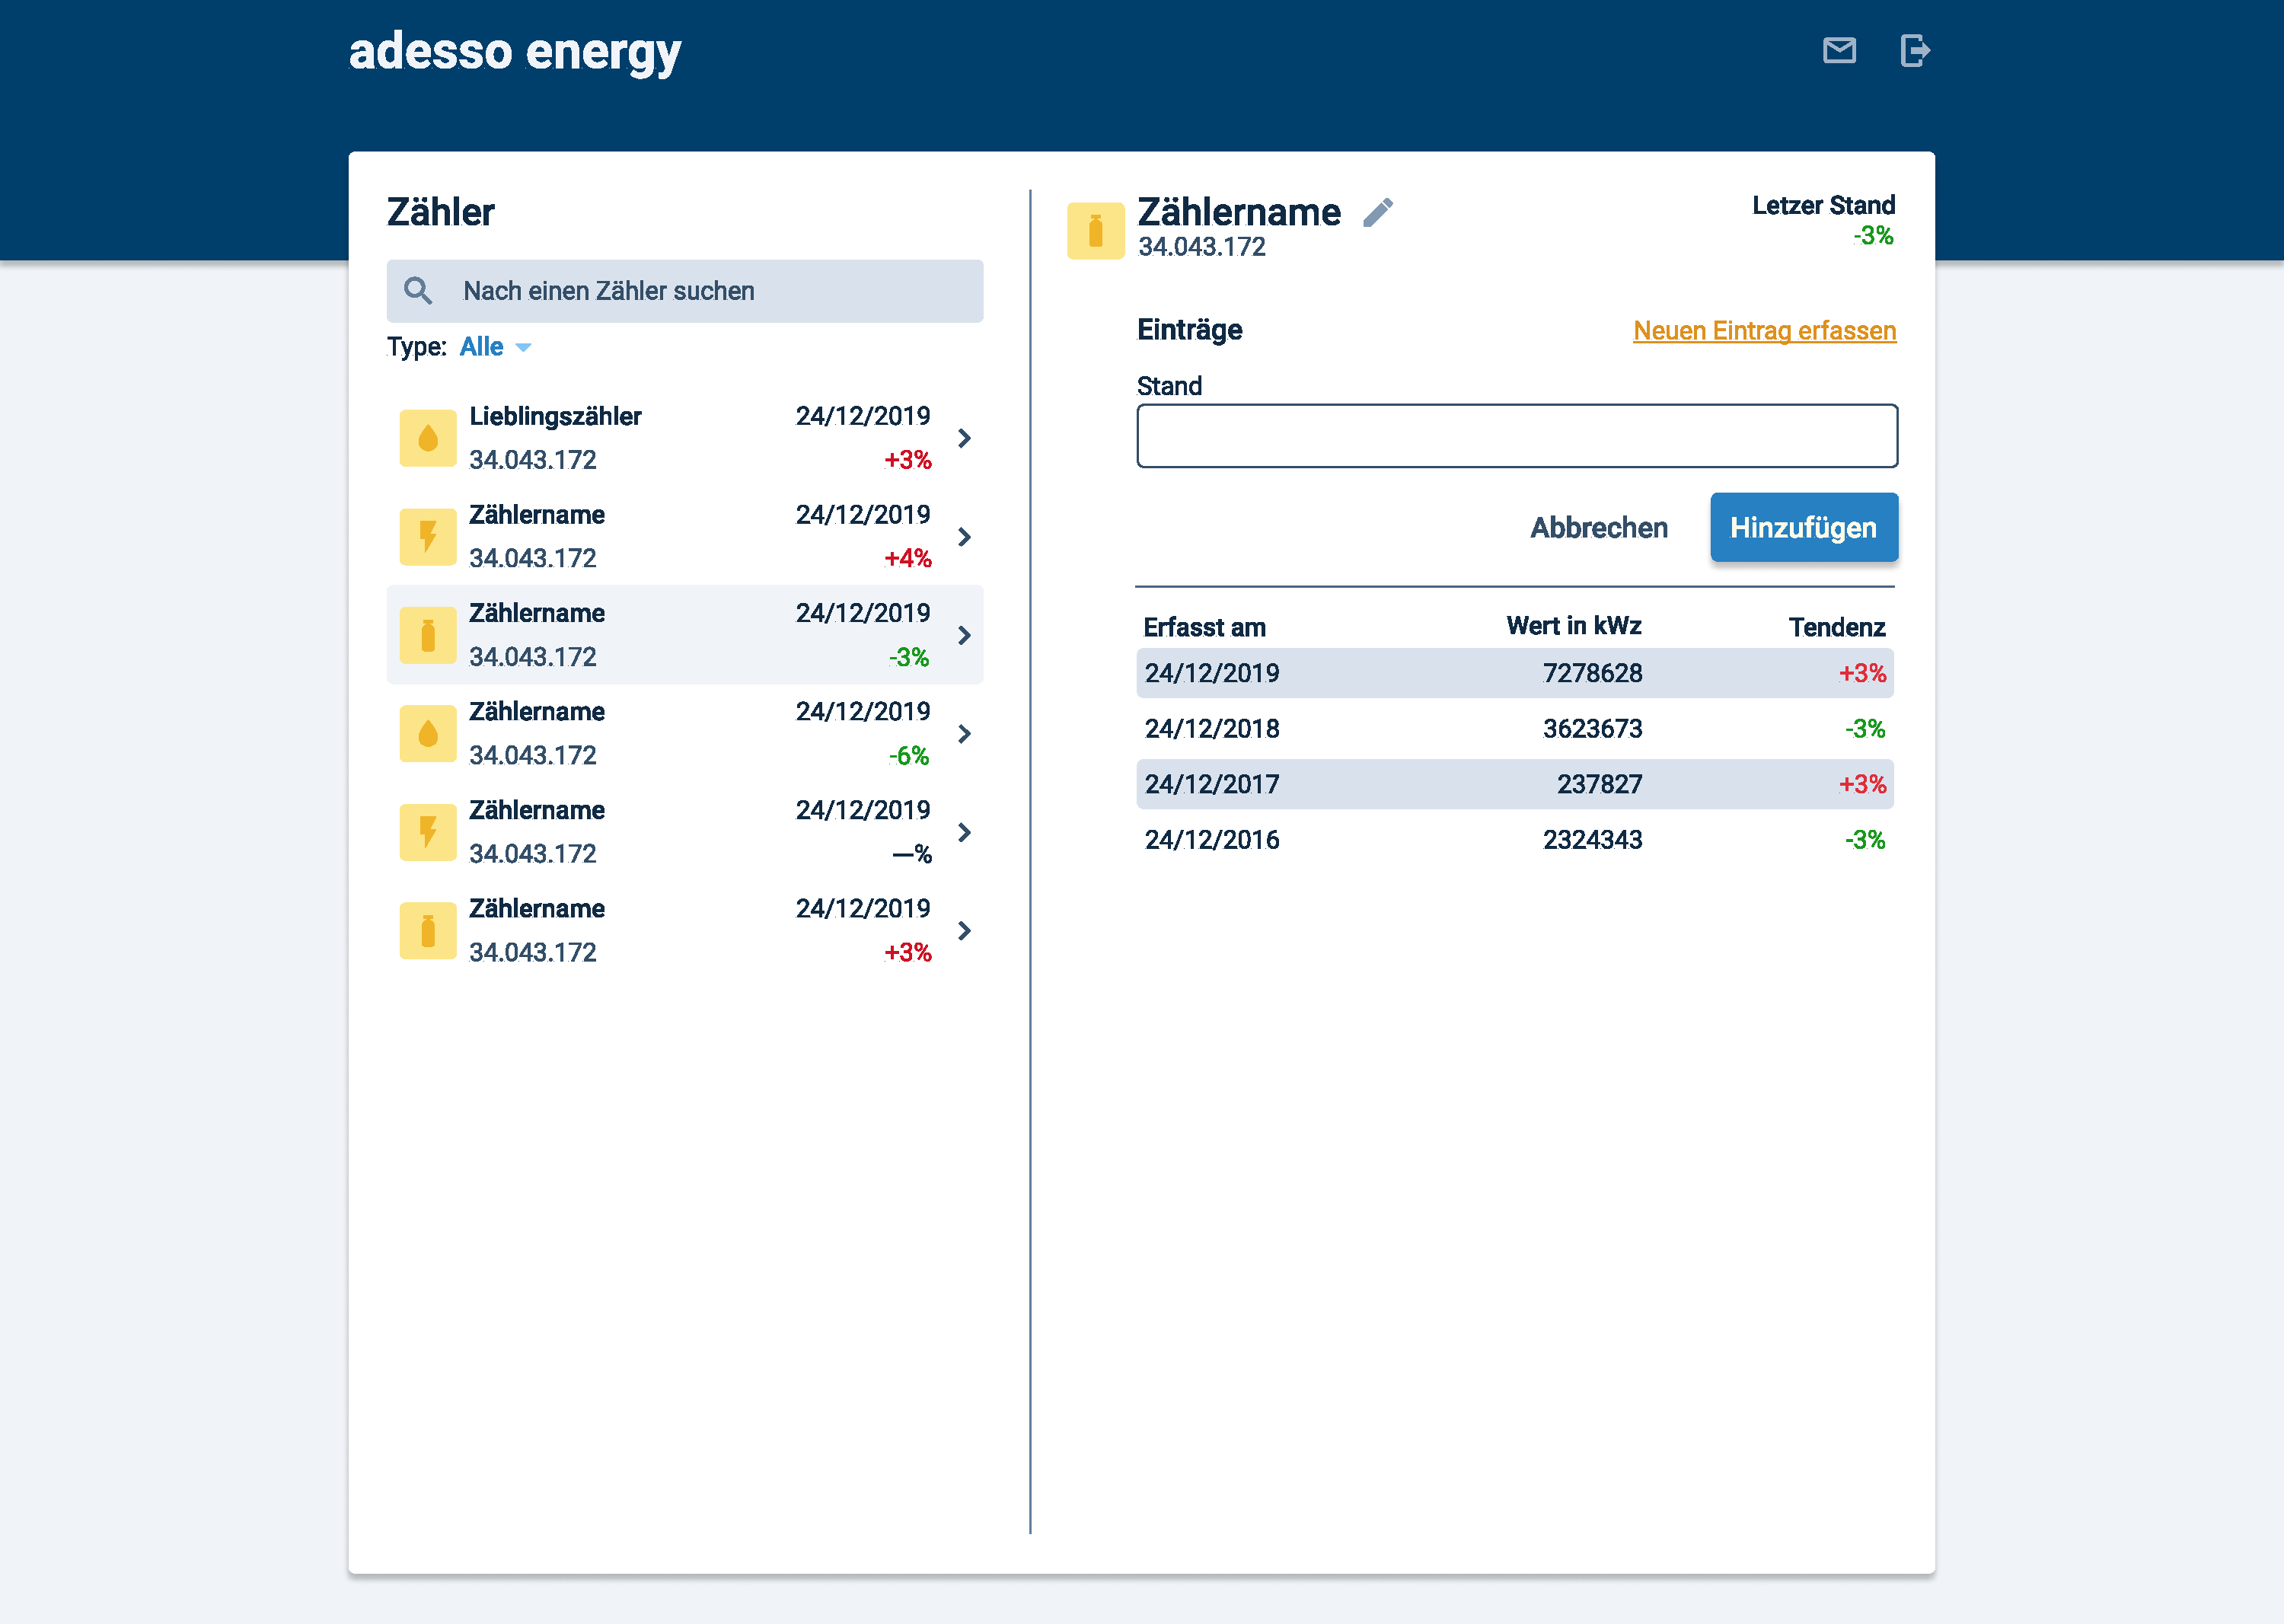
\includegraphics[scale=0.3]{img/WebsiteMockup/Dashboard-User-Selected-AddEntry}
	\caption{Dashboard User Eintrag hinzufügen} \hfill \break
	Nachdem man auf Neuen Eintrag erfassen klickt, wird ein Dialog angezeigt um einen neuen Stand festzuhalten.
\end{figure}

\newpage

\begin{figure}[h]
	\centering
    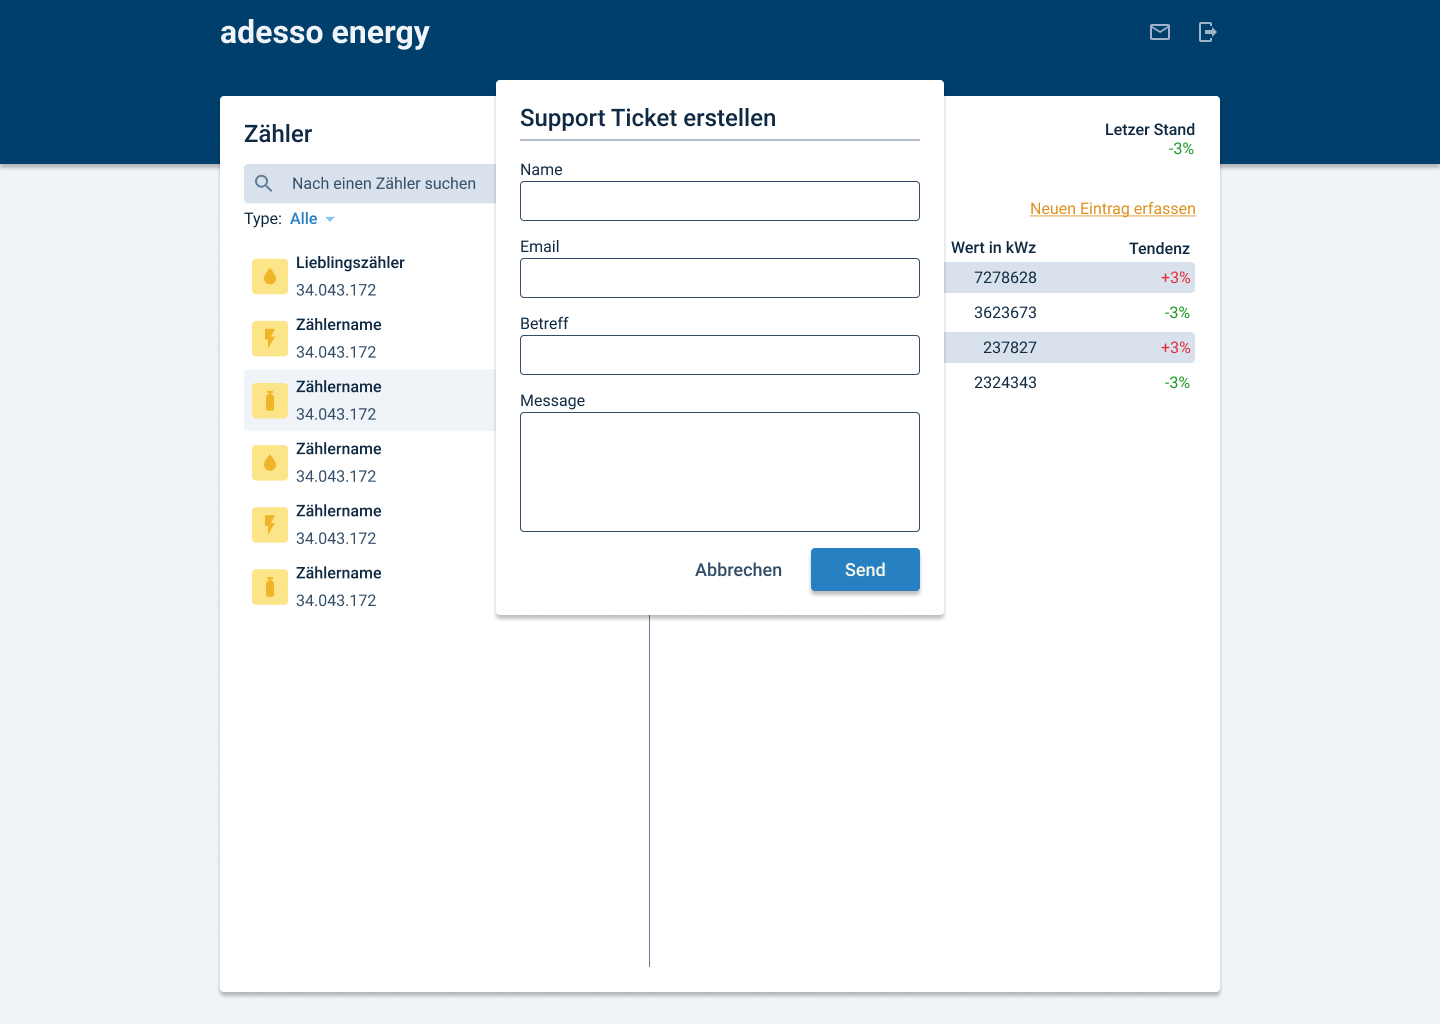
\includegraphics[scale=0.3]{img/WebsiteMockup/Dashboard-User-Mail}
	\caption{Dashboard User Support} \hfill \break
	Durch klicken auf das Mail Icon oben rechts auf der Seite wird ein Dialog zum erstellen eines neuen Support Tickets angezeigt.
\end{figure}

\newpage

\begin{figure}[h]
	\centering
    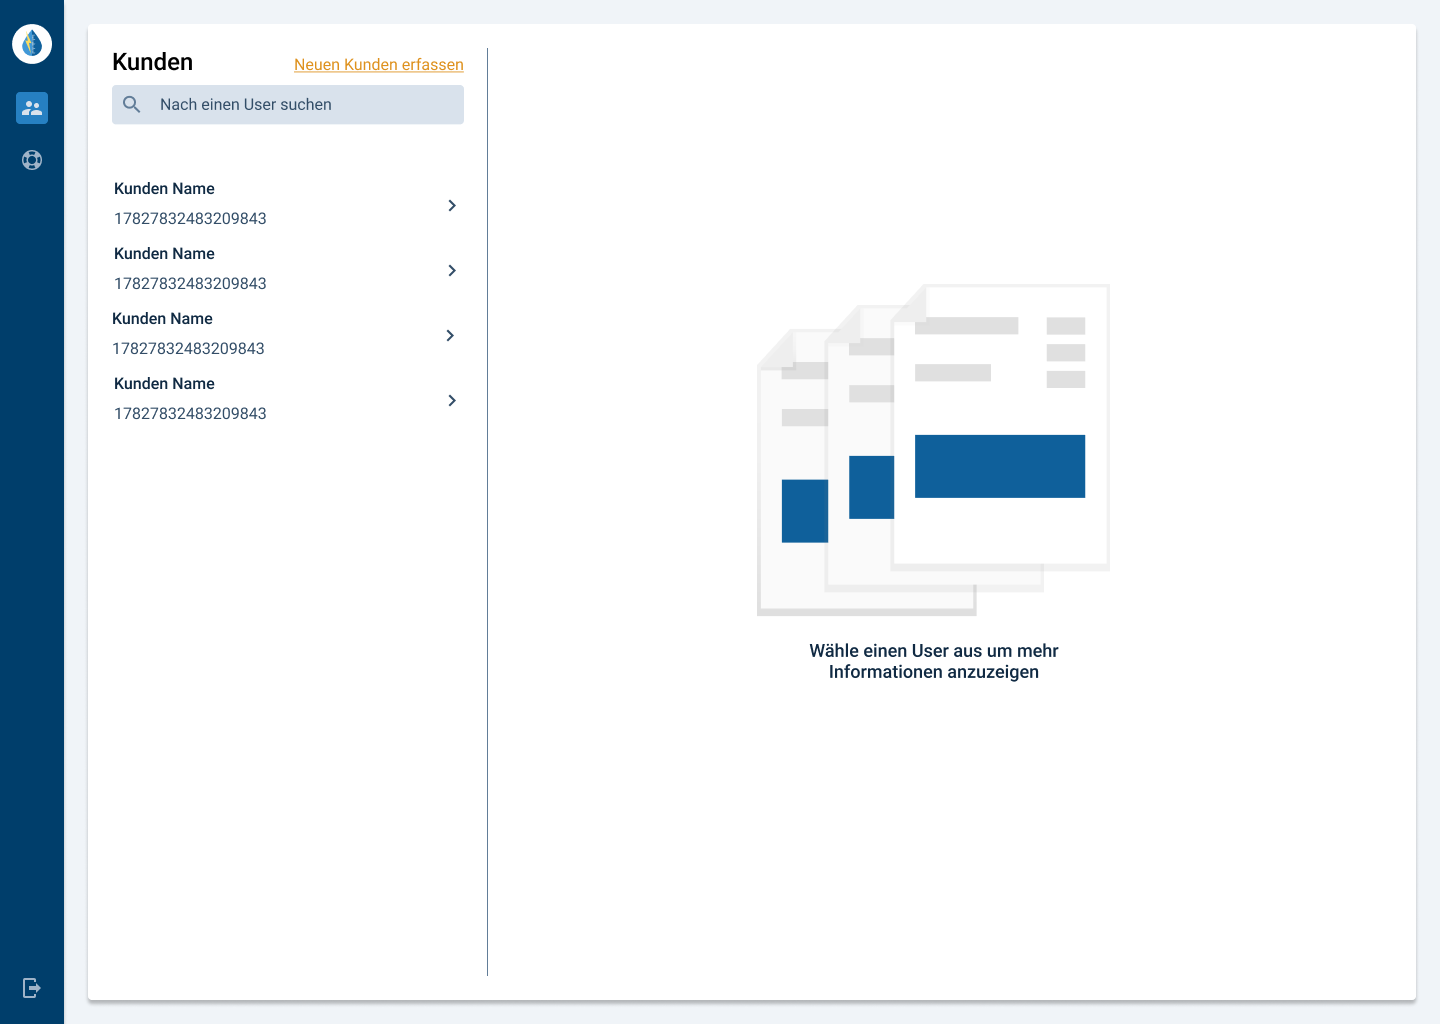
\includegraphics[scale=0.3]{img/WebsiteMockup/Dashboard-Admin-NonSelected}
	\caption{Dashboard Admin} \hfill \break
	Nachdem Login hat ein Administrator die Möglichkeit alle Kunden einzusehen.
\end{figure}

\newpage

\begin{figure}[h]
	\centering
    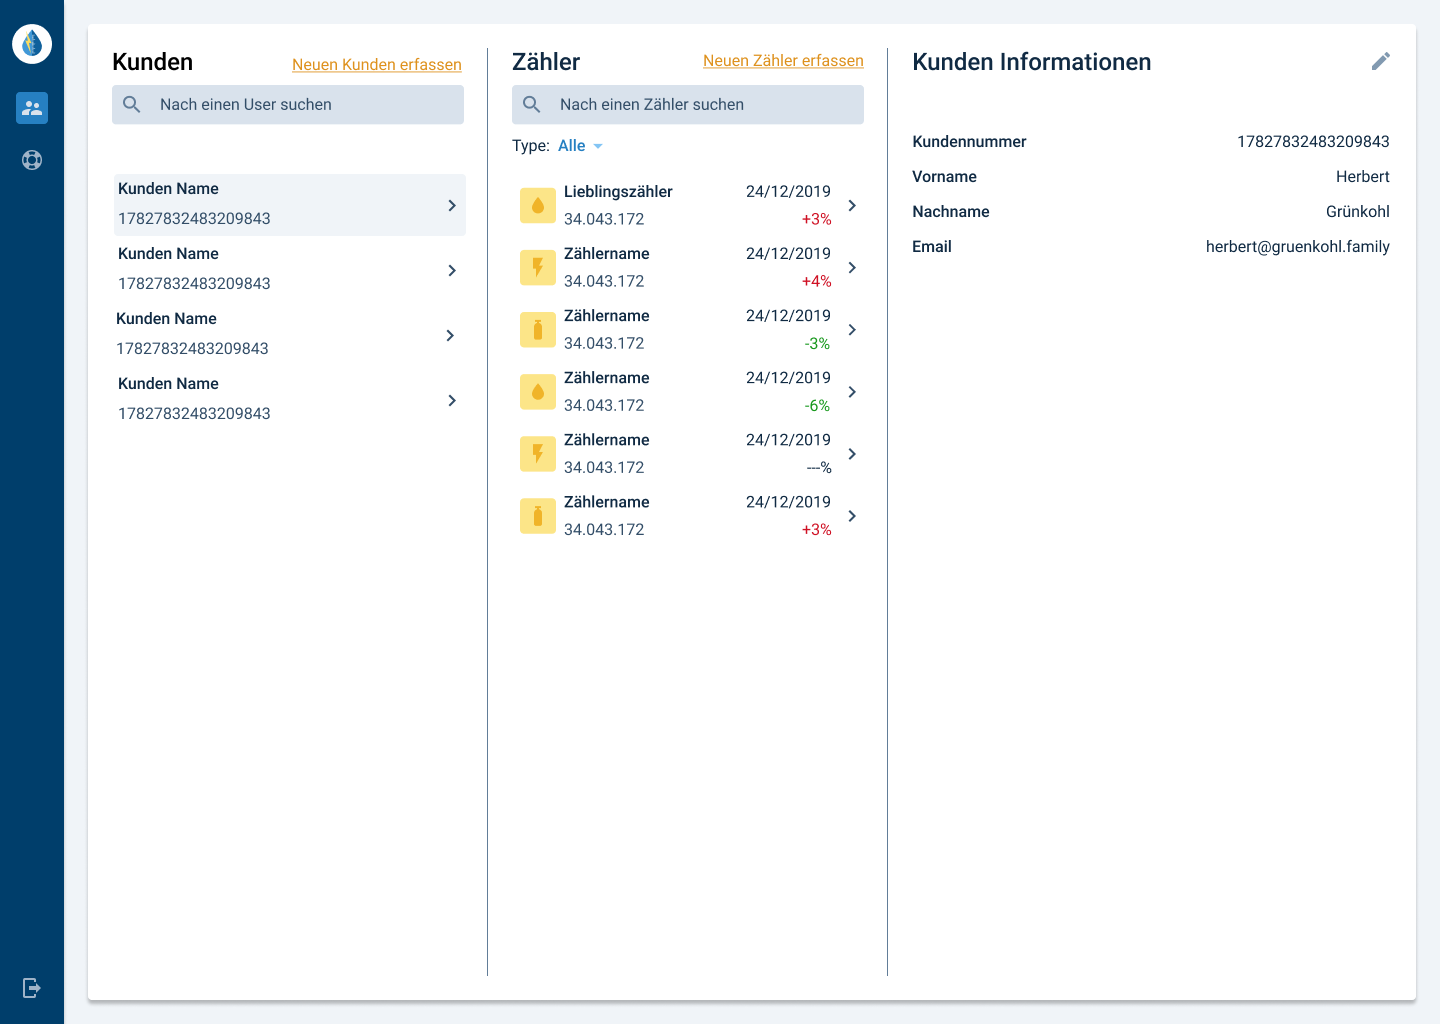
\includegraphics[scale=0.3]{img/WebsiteMockup/Dashboard-Admin-UserSelected}
	\caption{Dashboard Admin Benutzer ausgewählt} \hfill \break
	Nachdem der Administrator einen Kunden ausgewählt hat kann er die Informationen des Kunden einsehen.
\end{figure}

\newpage

\begin{figure}[h]
	\centering
    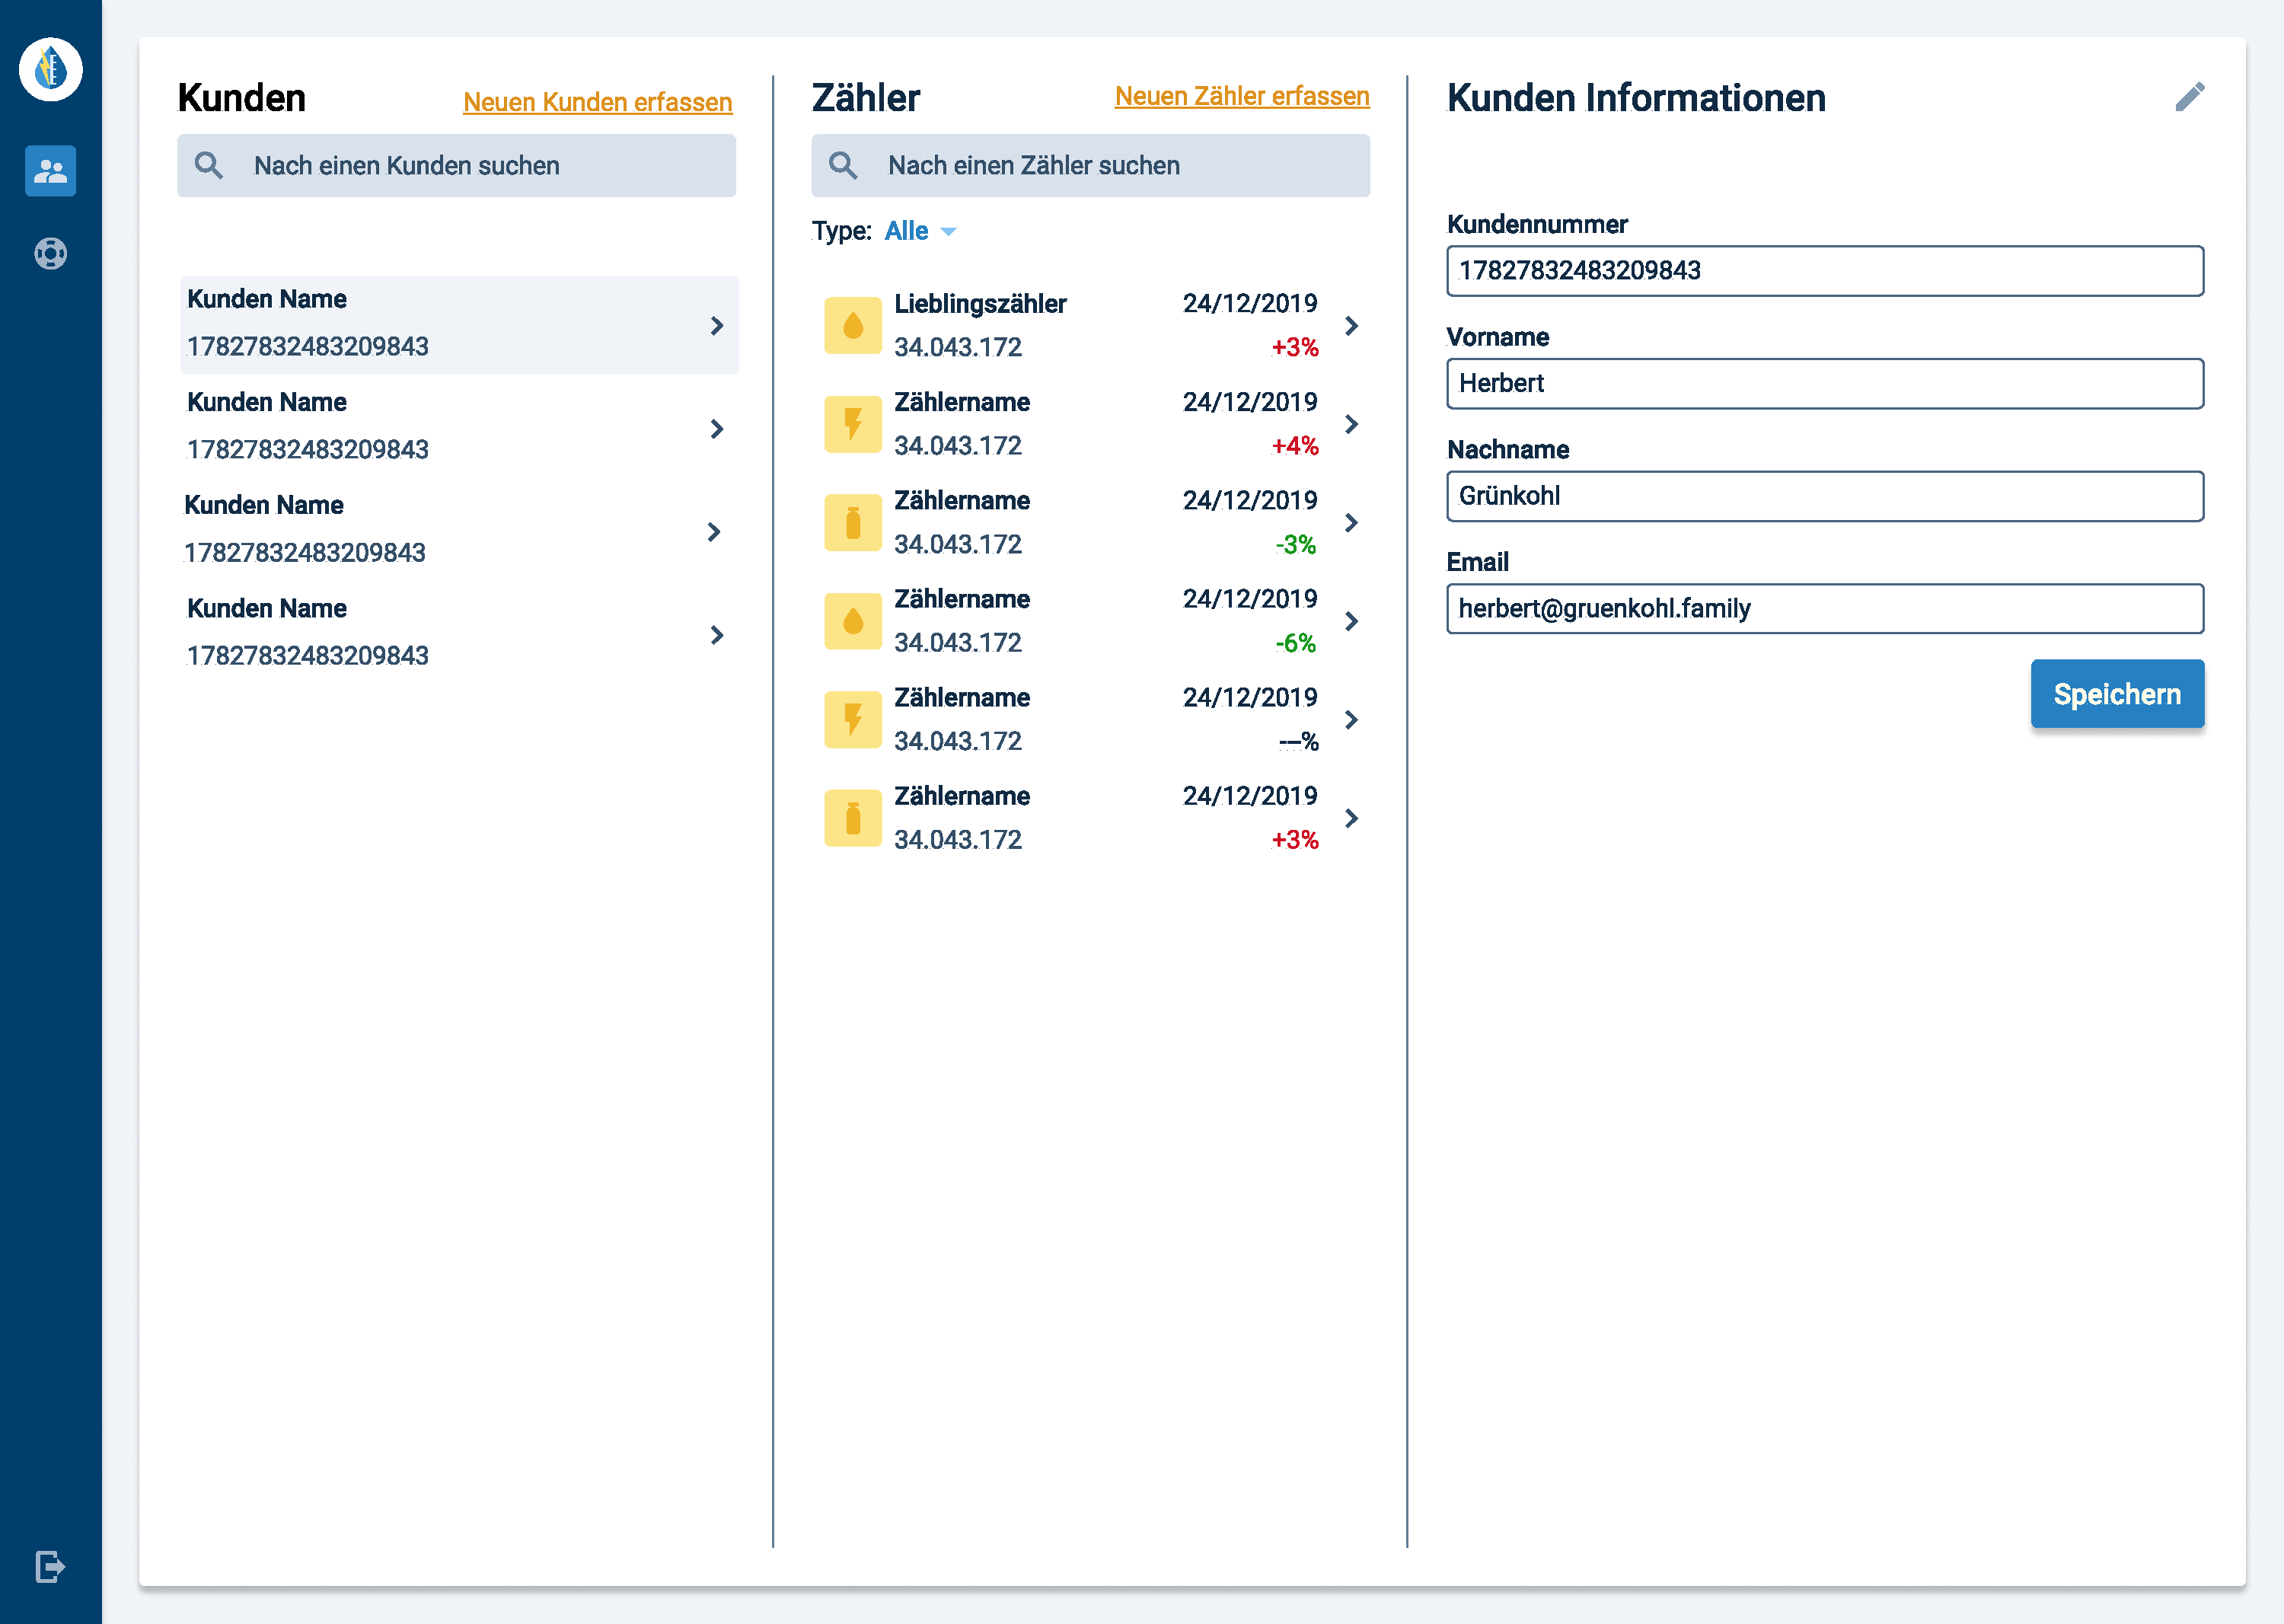
\includegraphics[scale=0.3]{img/WebsiteMockup/Dashboard-Admin-UserSelected-Edit}
	\caption{Dashboard Admin Benutzer editieren}\hfill \break
	Durch klicken des Stift Icons oben rechts auf der Seite kann ein Administrator den ausgewählten Kunden bearbeiten.
\end{figure}
\newpage

\begin{figure}[h]
	\centering
    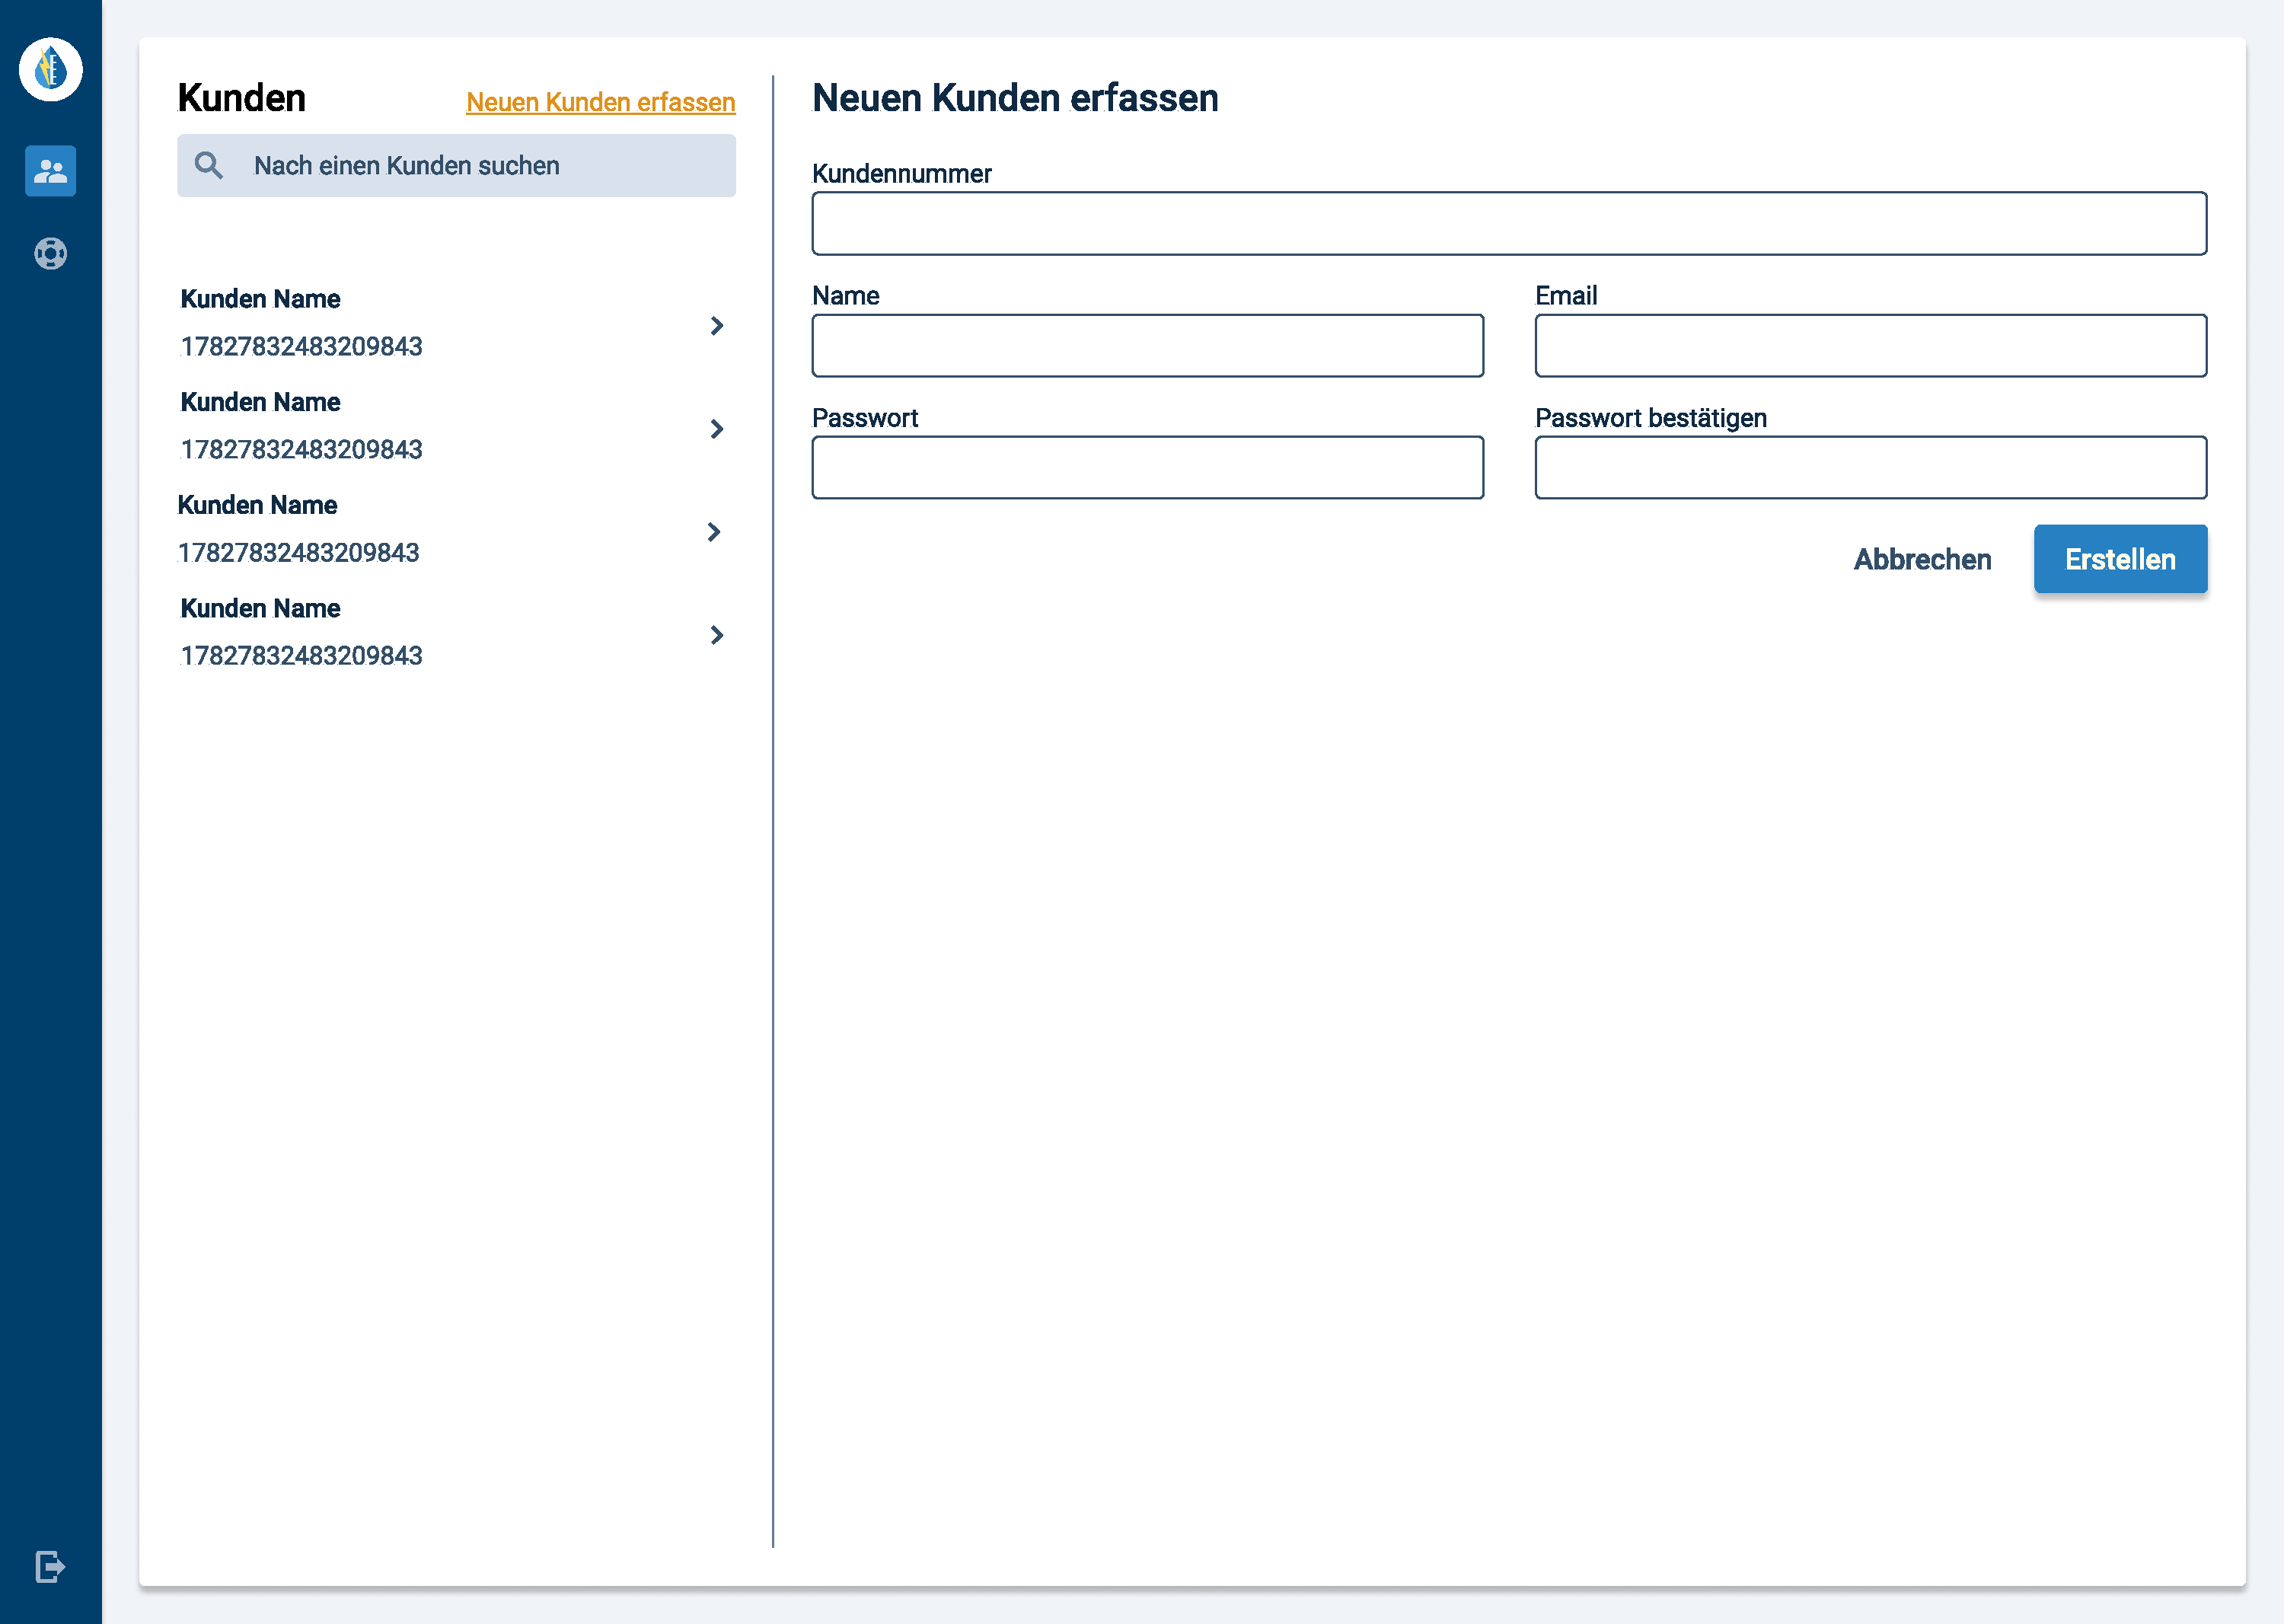
\includegraphics[scale=0.3]{img/WebsiteMockup/Dashboard-Admin-AddUser}
	\caption{Dashboard Admin Benutzer hinzufügen} \hfill \break
	Durch klicken auf Neuen Kunden erfassen kann der Administrator einen neuen Kunden zur Datenbank hinzufügen.
\end{figure}

\newpage

\begin{figure}[h]
	\centering
    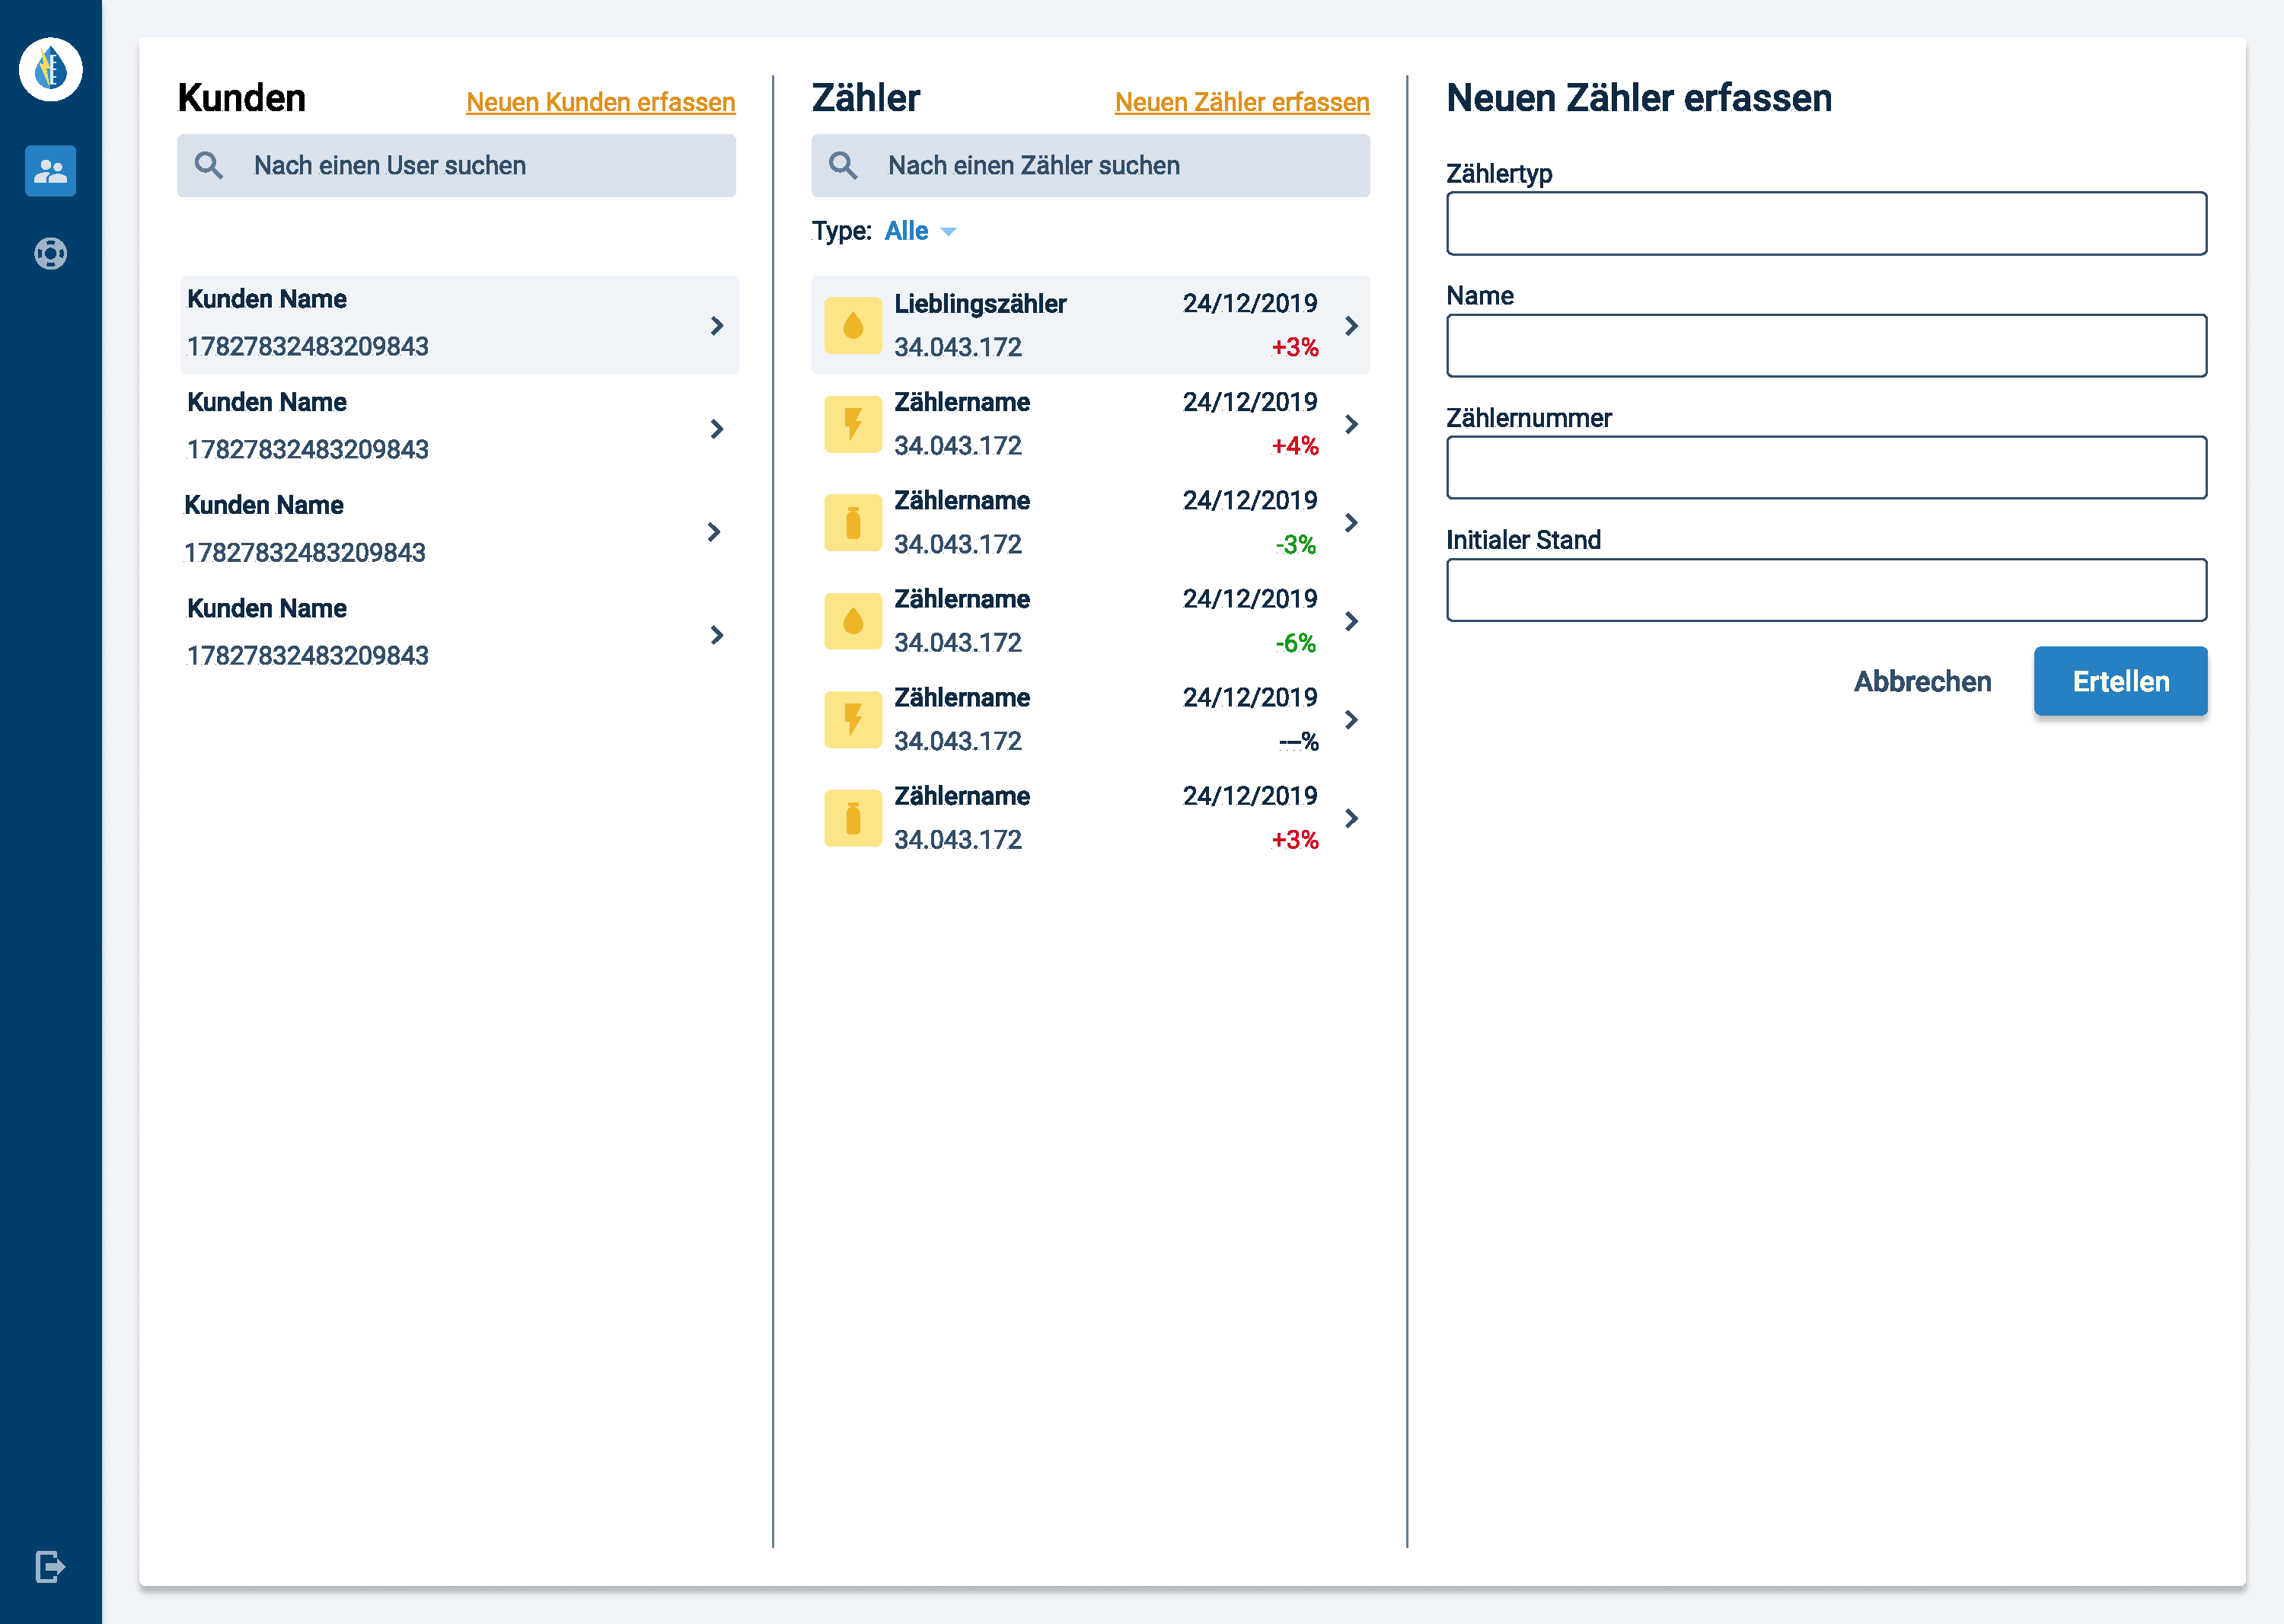
\includegraphics[scale=0.3]{img/WebsiteMockup/Dashboard-Admin-AddZahler}
	\caption{Dashboard Admin Zähler hinzufügen} \hfill \break
	Nachdem der Administrator einen Benutzer ausgewählt hat, kann er diesem einen neuen Zähler hinzufügen, indem er auf Neuen Zähler erfassen klickt.
\end{figure}

\newpage

\begin{figure}[h]
	\centering
    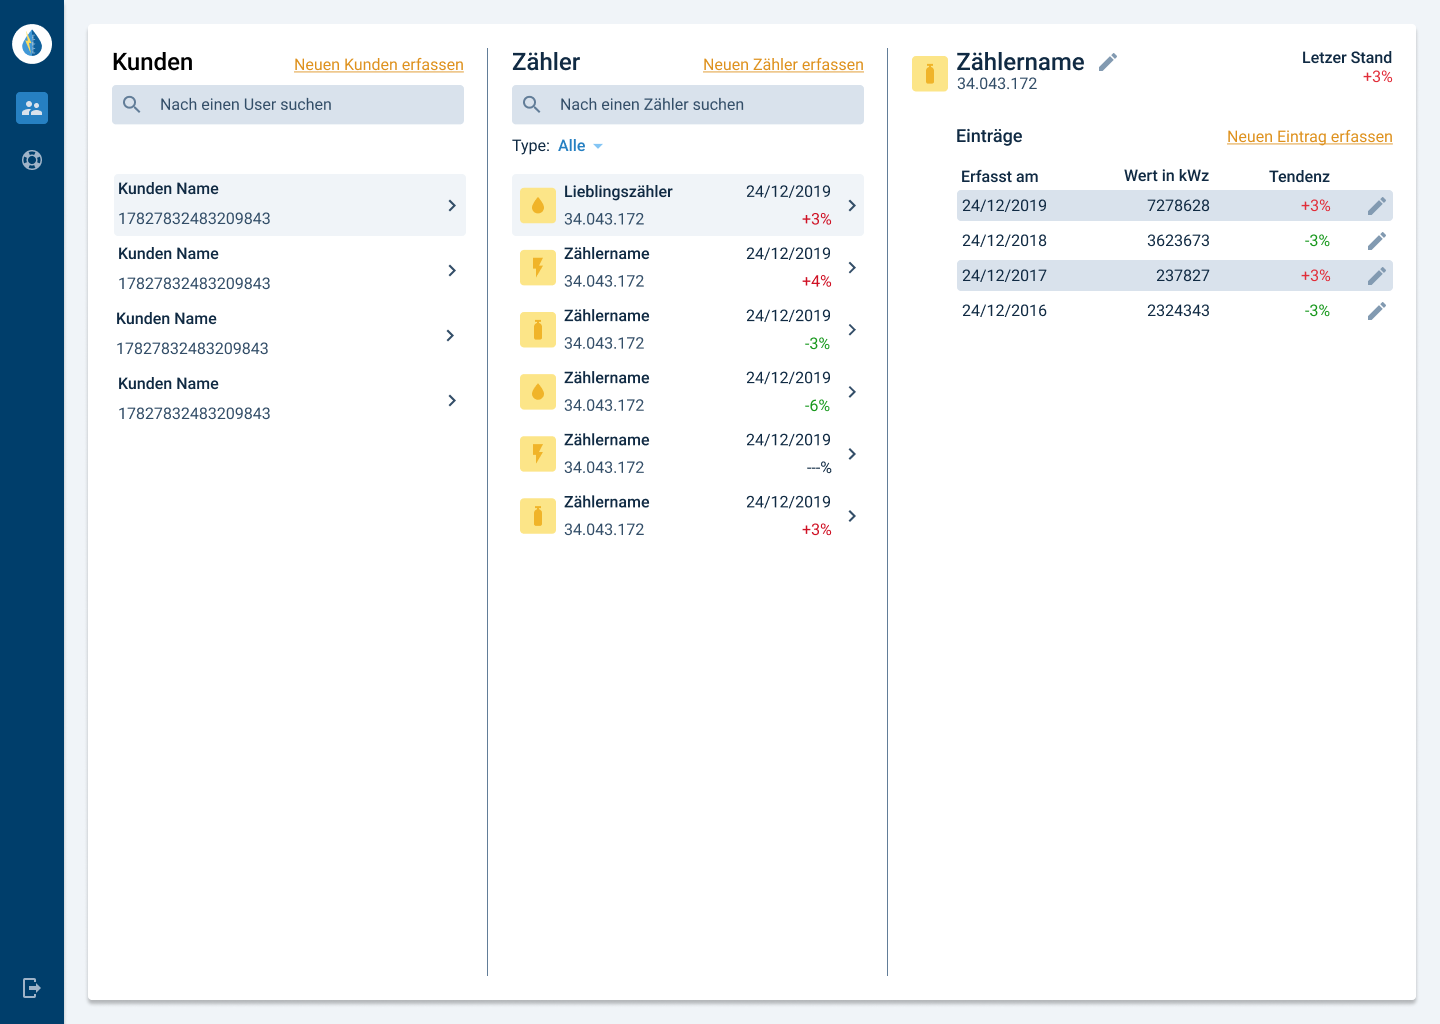
\includegraphics[scale=0.3]{img/WebsiteMockup/Dashboard-Admin-ZahlerSelected}
	\caption{Dashboard Admin Zähler ausgewählt} \hfill \break
	Nachdem der Adnimistrator auf einen Zähler geklickt hat, sieht er die Zählerinformation und History.
\end{figure}

\newpage

\begin{figure}[h]
	\centering
    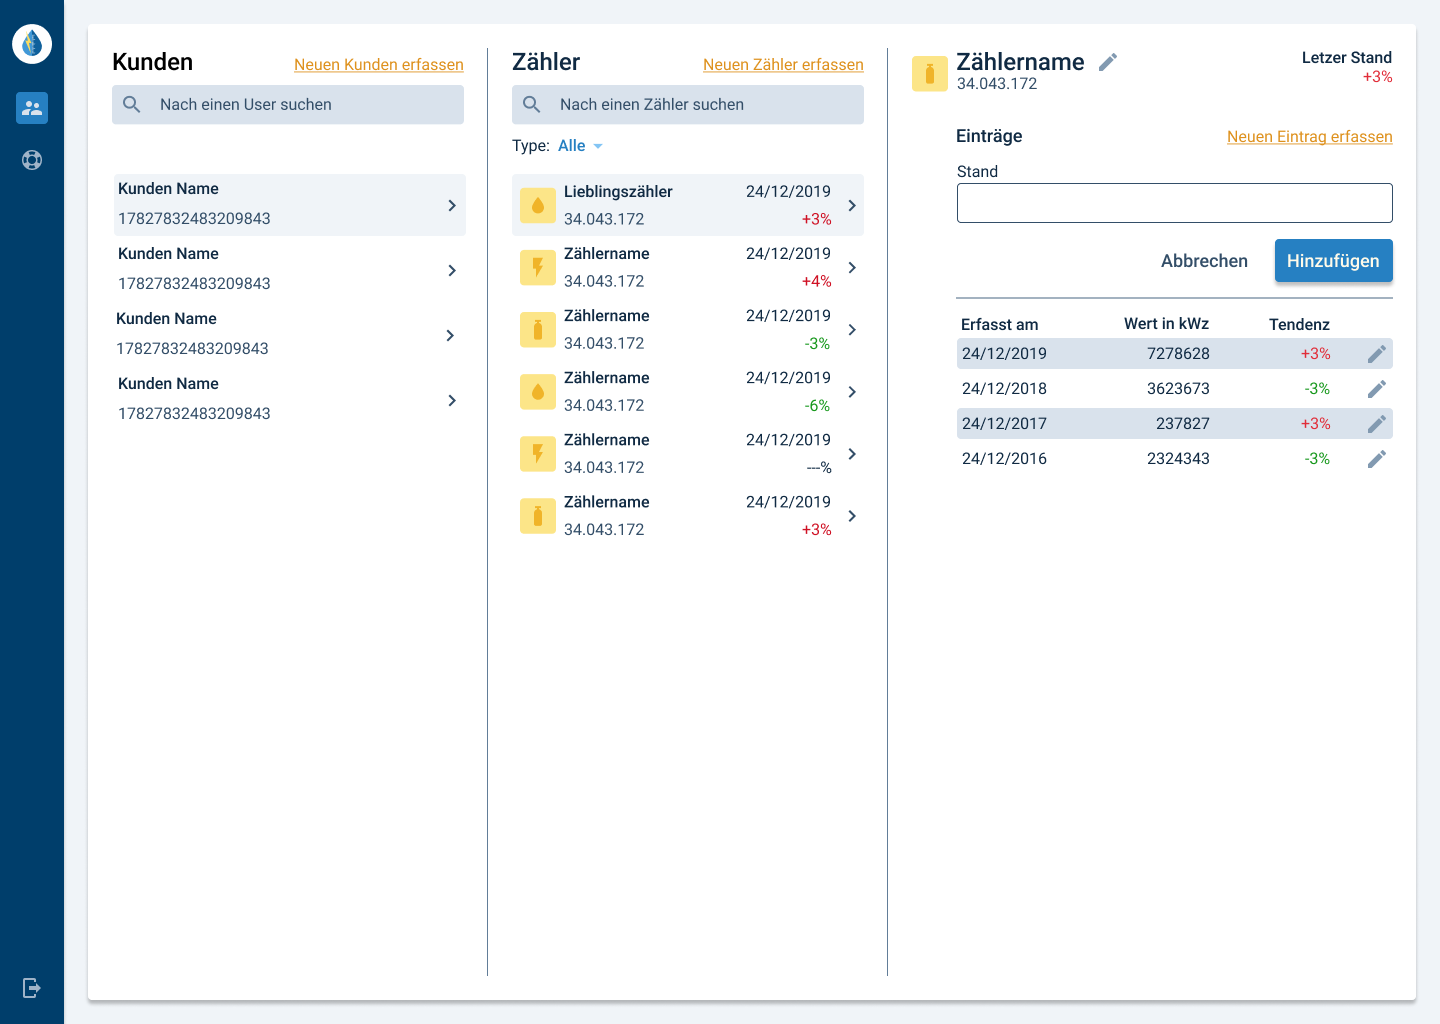
\includegraphics[scale=0.3]{img/WebsiteMockup/Dashboard-Admin-AddEntry}
	\caption{Dashboard Admin Eintrag hinzufügen} \hfill \break
	Wie auch der Benutzer hat der Admin auch die Möglichkeit Zählerstände einzutragen.
\end{figure}

\newpage

\begin{figure}[h]
	\centering
    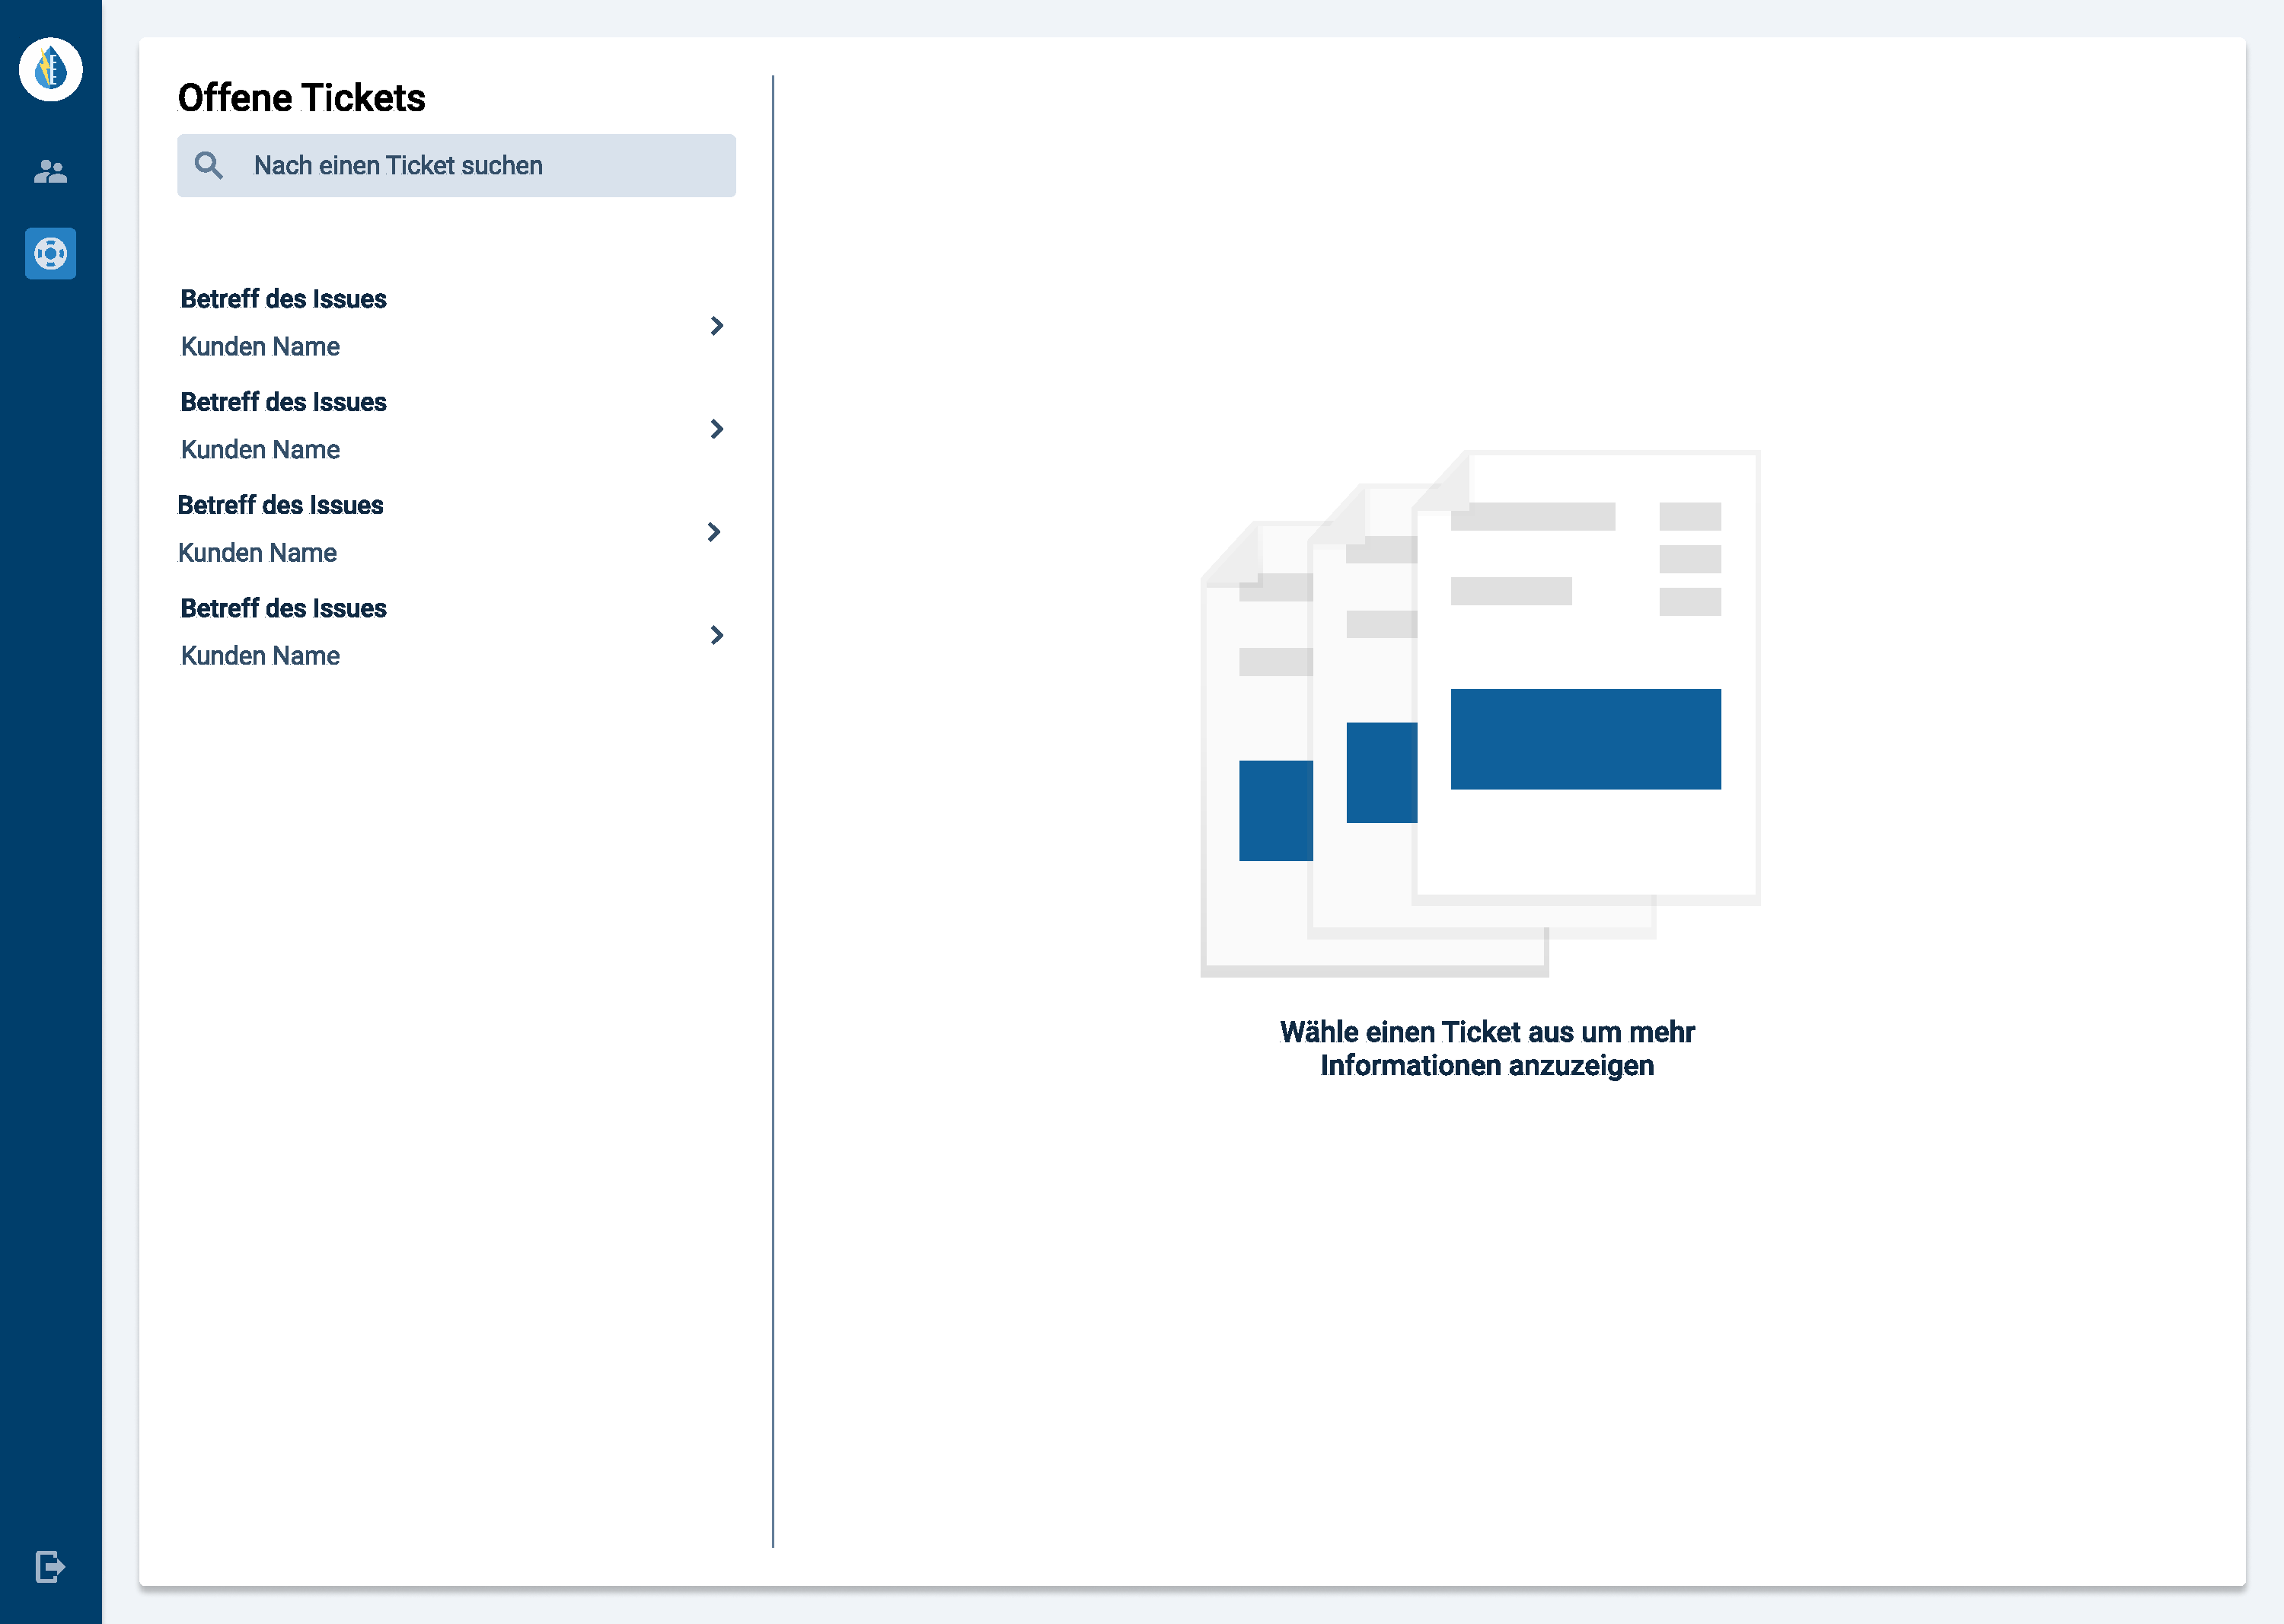
\includegraphics[scale=0.3]{img/WebsiteMockup/Dashboard-Admin-Support}
	\caption{Dashboard Admin Support} \hfill \break
	Nach dem klicken auf das Support Icon am linken Rand der Seite kann ein Administrator alle offenen Support Tickets einsehen.
\end{figure}

\newpage

\begin{figure}[h]
	\centering
    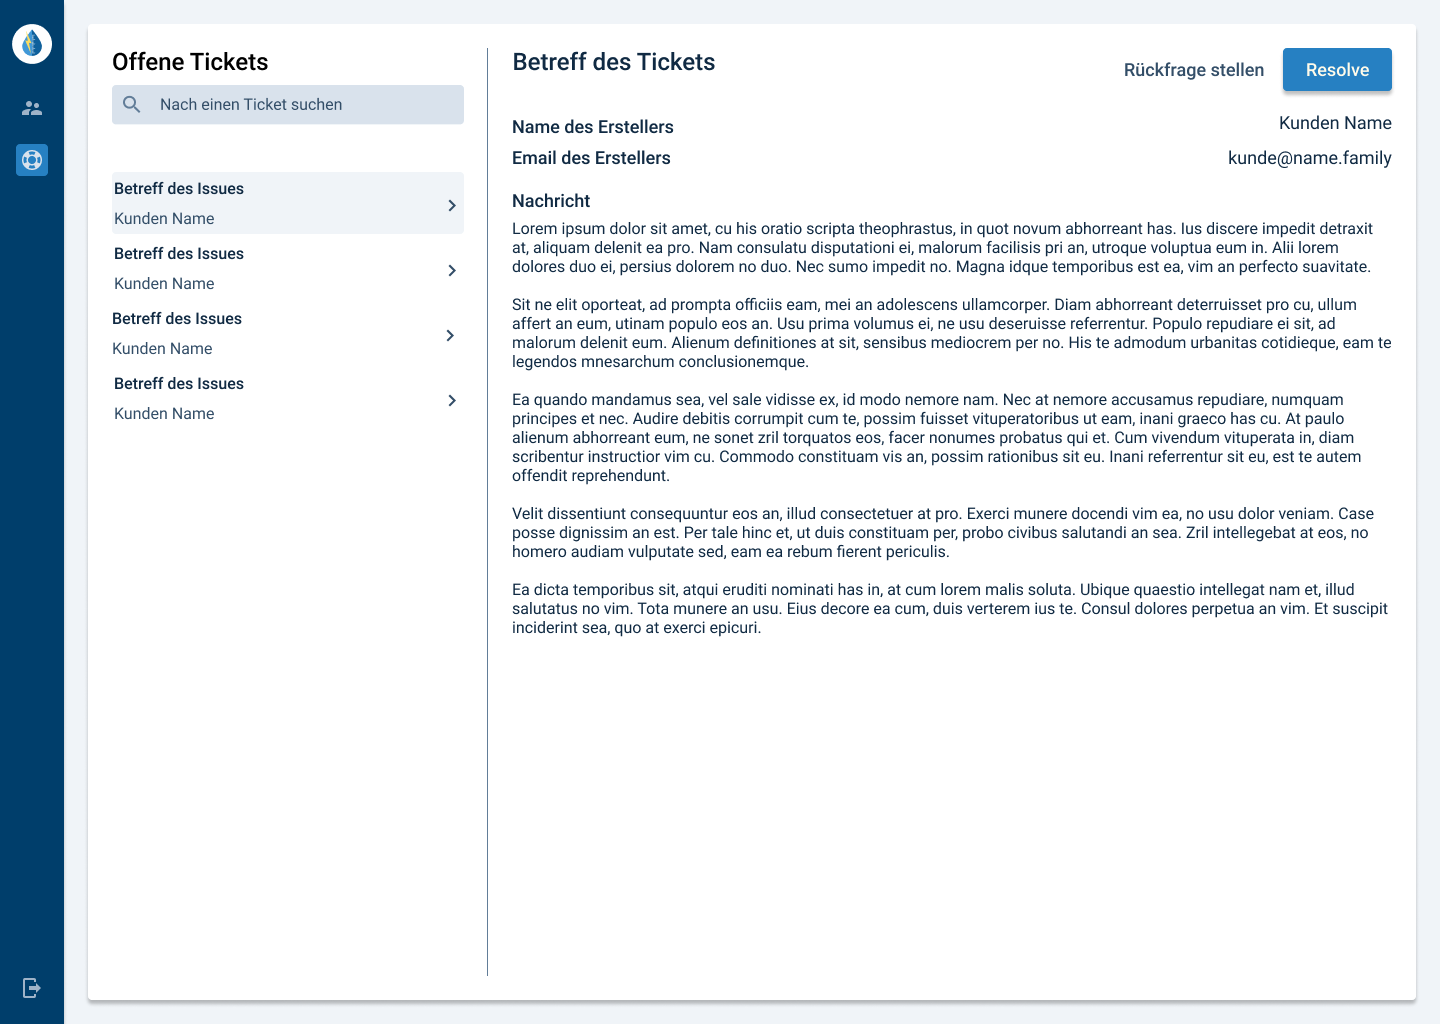
\includegraphics[scale=0.3]{img/WebsiteMockup/Dashboard-Admin-Support-Selected}
	\caption{Dashboard Admin Support Ticket ausgewählt} \hfill \break
	Durch auswählen einen Tickets kann der Administrator alle Information über das Ticket einsehen, das Ticket schließen, oder Rückfragen stellen.
\end{figure}

